% vim:spell spelllang=en:
\documentclass[a4paper,11pt]{book}
\usepackage[utf8]{inputenc}
%\usepackage{fullpage}
\usepackage{listings}
\usepackage{color}
\usepackage{url}
\usepackage{alltt}
\usepackage{multicol}
\usepackage{fancyhdr}
\usepackage{amsmath}
\usepackage{bussproofs}
\usepackage{comment}
\usepackage{inconsolata}
\usepackage{graphicx}

\usepackage{hyperref}
\definecolor{darkgreen}{rgb}{0.0,0.5,0.0}
\hypersetup{colorlinks=true,citecolor=darkgreen}

\renewcommand{\familydefault}{\sfdefault} % change to sans serif font

\newcommand{\seq}{\vdash}	% the sequent sign
\newcommand{\impl}{\supset} %logical connectives: implies, not, and, or
\renewcommand{\lnot}{\neg}
\renewcommand{\land}{\wedge}
\renewcommand{\lor}{\vee}
\newcommand{\sklabel}[2]{\langle#1\rangle^{#2}}
\newcommand{\LK}{\textbf{LK}}
\newcommand{\ND}{\textbf{ND}}
\newcommand{\unsubst}[2]{[{#1}\backslash{#2}]}	% a unary substitution like, e.g., [x\t]

%Commands for constructing proof trees with bussproofs. See the chapter on the LK system for examples.
\newcommand{\UnaryInfCm}[1]{\UnaryInfC{$#1$}}
\newcommand{\BinaryInfCm}[1]{\BinaryInfC{$#1$}}
\newcommand{\TrinaryInfCm}[1]{\TrinaryInfC{$#1$}}
\newcommand{\RightLabelm}[1]{\RightLabel{$#1$}}
\newcommand{\AxiomCm}[1]{\AxiomC{$#1$}}

% Normal text in math mode ("math text")
\newcommand{\mt}[1]{\textnormal{#1}}
% CLI-style names,words,... within normal text
\newcommand{\cli}[1]{{\ttfamily {#1}}}

\usepackage[draft]{fixme}
\fxsetup{inline,nomargin,marginclue,theme=color,index}

\lstset{
  basicstyle=\small\ttfamily,
  breaklines=true,
%
  frame=leftline,
  framesep=1ex,
  framerule=1ex,
  rulecolor={\color[rgb]{0.8,0.8,0.8}},
%
  inputencoding=utf8,
  extendedchars=true,
  columns=flexible,
  upquote=true,
  morecomment=[l][\bfseries]{gapt> },
  literate=%
    % FIXME: figure out why the Unicode symbols "eat" their trailing spaces
    {⊥}{{\ensuremath{\bot}} }1%
    {⊤}{{\ensuremath{\top}} }1%
    {∧}{{\ensuremath{\land}} }1%
    {⊃}{{\ensuremath{\impl}} }1%
    {∨}{{\ensuremath{\lor}} }1%
    {¬}{{\ensuremath{\neg}} }1%
    {→}{{\ensuremath{\rightarrow}} }1%
    {∀}{{\ensuremath{\forall}}}1%
    {∃}{{\ensuremath{\exists}}}1%
    {⊢}{{\ensuremath{\vdash}} }1%
    {ι}{{\ensuremath{\iota}}}1%
    {α}{{\ensuremath{\alpha}}}1%
    {β}{{\ensuremath{\beta}}}1%
    {τ}{{\ensuremath{\tau}}}1%
    {λ}{{\ensuremath{\lambda}}}1%
    {∈}{{\ensuremath{\in}}}1%
  }

% = clilisting environment
%
% This environment contains CLI interactions which are automatically evaluated
% using "sbt evalUserManual".
%
% Usage:
%
% \begin{clilisting}
% gapt> true
% res1: Boolean = true
% \end{clilisting}
%
% \begin{clilisting}[someCondition]
% gapt> this will only be executed if someCondition returns true
% \end{clilisting}
%
\lstnewenvironment{clilisting}[1][]{}{}

\lstdefinelanguage{scala}{
  morekeywords={abstract,case,catch,class,def,%
    do,else,extends,false,final,finally,%
    for,if,implicit,import,match,mixin,%
    new,null,object,override,package,%
    private,protected,requires,return,sealed,%
    super,this,throw,trait,true,try,%
    type,val,var,while,with,yield},
  otherkeywords={=>,<-,<\%,<:,>:,\#,@},
  sensitive=true,
  showstringspaces=false,
  morecomment=[l]{//},
  morecomment=[n]{/*}{*/},
  morestring=[b]",
  morestring=[b]',
  morestring=[b]"""
}

\lstnewenvironment{tacticslisting}[1][]{\lstset{language=scala}}{}
\lstnewenvironment{tacticsoutput}{}{}

\setlength{\parindent}{0pt}
\setlength{\parskip}{4pt}
\setlength{\headheight}{14pt}
\setlength{\oddsidemargin}{1pt}
\setlength{\evensidemargin}{1pt}
\setlength{\textwidth}{450pt}
%\setlength{\textheight}{600pt}

\pagestyle{fancy}
\lhead{GAPT -- User Manual}
\chead{}
\rhead{}
\cfoot{\thepage}

\begin{document}
\begin{titlepage}
\begin{center}

\hrule

\vspace*{20mm}

{\Huge GAPT}

\vspace*{5mm}

{\huge General Architecture for Proof Theory}

\vspace*{20mm}

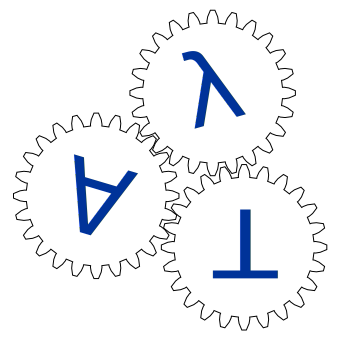
\includegraphics[keepaspectratio,width=5cm]{logo}

\vspace*{20mm}

{\Huge User manual}

\vspace*{10mm}
{\Large Version 2.9-SNAPSHOT}
\vspace*{10mm}

{\Large \today}

\vspace*{20mm}

\hrule
\end{center}

\end{titlepage}

\listoffixmes

\setcounter{tocdepth}{1}
\tableofcontents

\chapter{Introduction}

GAPT is a general architecture for proof theory implemented in Scala.
The focus of GAPT are proof transformations (in contrast to proof assistants,
whose focus is proof formalization, and automated deduction systems, whose focus
is proof search). GAPT is used from a shell that provides access to the functionality
in the system in a way that is inspired by computer algebra systems: the basic
objects are formulas and (different kinds of) proofs which can be modified
by calling GAPT commands from the command line. In addition, there
is a graphical user interface that allows the user to view (and—to a certain extent—
modify) proofs in a flexible and visually appealing way.

The current functionality of GAPT includes data structures for formulas,
sequents, resolution proofs, sequent calculus proofs, expansion tree proofs and
algorithms for e.g.\ unification, proof Skolemization, cut-elimination, cut
elimination by resolution~\cite{Baaz00CutElimination},
cut-introduction~\cite{Hetzl2012}, etc. It contains a built-in superposition
prover, an inductive theorem prover, as well as interfaces to numerous external
theorem provers and solvers.

This user manual is an introduction to the usage of GAPT, mostly based on examples.
We recommend that you try out these examples in your installation of GAPT while
reading this manual.

\chapter{Download and execution}

There are three ways you can obtain GAPT:

\begin{enumerate}

\item {\bfseries The recommended way:}  You can download a package of the current
version of GAPT at~\url{https://logic.at/gapt/}.  After extracting
the \texttt{tar.gz}-file, you will find a shell script \texttt{gapt.sh}.

Running this script will start the command line interface of GAPT:
\begin{lstlisting}
./gapt.sh
\end{lstlisting}

\item If you are adventurous, you can also download the current development
  version from github:
\begin{lstlisting}
git clone https://github.com/gapt/gapt
cd gapt
sbt console
\end{lstlisting}

\item If you like GAPT and want to use it as a library in your Scala project,
  it is available as a Maven artifact on JCenter.  All you need to do is add
  two lines to your \verb,build.sbt,:
\begin{lstlisting}
resolvers += Resolver.jcenterRepo
libraryDependencies += "at.logic.gapt" %% "gapt" % "2.8"
\end{lstlisting}

\end{enumerate}

The command line interface of GAPT is an interactive Scala shell.  This means
that all functionality of Scala is available to you.  In particular it is easy
to write Scala scripts that use the functionality of GAPT.

You don't need to know anything about Scala to try out the examples in this
manual, but if you do want to learn more about Scala we recommend the book
``Programming in Scala''~\cite{odersky2008programming}.

Interactions with the Scala shell are typeset in the following way:
\begin{clilisting}
gapt> println("Hello, world!")
Hello, world!

\end{clilisting}
Here, {\bfseries \cli{println("Hello, world!")}} is the user input, and \texttt{Hello,
world!} is the output from the Scala shell.

If you want to consult the in-depth API documentation of a function, you can
use the \cli{help} command:
\begin{clilisting}
gapt> help(containsQuantifierOnLogicalLevel)

\end{clilisting}

\section{Required and optional software}
\label{sec:sysreq}

To run GAPT you need to have Java 8 (or higher) installed.

GAPT contains interfaces to the following automated reasoning systems. Installing
them is optional. If GAPT does not find the executables in the path, the
functionality of these systems will not be available.

\begin{itemize}
\item Prover9 (\url{http://www.cs.unm.edu/~mccune/mace4/download/}) - make sure
  the commands \texttt{prover9} and \texttt{prooftrans} are available.
\item E theorem prover (\url{http://eprover.org/})
\item Vampire 4.0 (\url{http://www.vprover.org/})
\item SPASS (\url{http://www.spass-prover.org/})
\item LeanCoP (\url{http://leancop.de/})
\item Metis (\url{http://www.gilith.com/software/metis/})
\item iProver (\url{http://www.cs.man.ac.uk/~korovink/iprover/}, requires
  a development version as of September 11, 2017)
\item VeriT (\url{http://www.verit-solver.org/})
\item Z3 (\url{https://github.com/Z3Prover/z3})
\item MiniSAT (\url{http://minisat.se/})
\item Glucose (\url{http://www.labri.fr/perso/lsimon/glucose/})
\item PicoSAT (\url{http://fmv.jku.at/picosat/})
\item Sat4J (\url{http://sat4j.org/})
\item OpenWBO (\url{http://sat.inesc-id.pt/open-wbo/})
\item CVC4 (\url{http://cvc4.cs.nyu.edu/web/})
\item TIP tools (\url{https://github.com/tip-org/tools})
\end{itemize}

\chapter{Data structures}

\section{Expressions and formulas}

Formulas, terms, and all other expressions are represented as terms in a
polymorphic simply-typed lambda calculus. GAPT's lambda calculus also supports
multiple base sorts and inductive types, see Appendix~\ref{ch.lamda_calculus}
for a complete definition. For example, the formula $\forall
x\: P(x, y)$ is encoded as the term \cli{'$\forall$' ($\lambda$x (P x) y)}.
This term has the type $o$, which is the type of Boolean values.  The variable
$x$ in this term has the type $i$, which is the default type for first-order
variables.

There are two ways of entering expressions: you can parse them or construct them
manually.

\subsection{Formula parsing}
Here is an example of parsing a first-order formula:
\begin{clilisting}
gapt> val F = fof"!x (P(x,f(x)) -> ?y P(x,y))"
F: at.logic.gapt.expr.FOLFormula = ∀x (P(x, f(x)) ⊃ ∃y P(x, y))

\end{clilisting}

Every kind of expression that GAPT supports can be parsed by writing \verb!<prefix>"<string>"!.
The prefix indicates the Scala type of the expression. The following prefixes are available:

\begin{tabular}{r l}
\cli{ty} & type \\
\cli{le} & lambda expression \\
\cli{hof} & higher-order formula \\
\cli{hoa} & higher-order atom \\
\cli{hov} & higher-order variable \\
\cli{hoc} & higher-order constant \\
\cli{foe} & first-order expression \\
\cli{fof} & first-order formula \\
\cli{fot} & first-order term \\
\cli{foa} & first-order atom \\
\cli{fov} & first-order variable \\
\cli{foc} & first-order constant
\end{tabular}

This parser supports Scala string interpolation. For example, you can do:
\begin{clilisting}
gapt> val t = fot"f(f(x))"
t: at.logic.gapt.expr.FOLTerm = f(f(x))

gapt> val G = fof"!x (P(x,$t) -> ?y P(x,y))"
G: at.logic.gapt.expr.FOLFormula = ∀x (P(x, f(f(x))) ⊃ ∃y P(x, y))

\end{clilisting}

Note that Scala string interpolation is different from (capture-avoiding) substitution.

The input language has full type inference, and the formula
prefixes make sure that the expression is of type $o$ (Boolean).  If no
particular type is required, we default to $\iota$:
\begin{clilisting}
gapt> hof"!x?y!z x(z) = y(y(z))"
res2: at.logic.gapt.expr.Formula = ∀x ∃y ∀z x(z) = y(y(z))

\end{clilisting}

So far we have only used the ASCII-safe part of the syntax, however Unicode
input is of course supported as well---you can paste any of the output right
back in:
\begin{clilisting}
gapt> hof"∀x ∃y ∀z x(z) = y(y(z))"
res3: at.logic.gapt.expr.Formula = ∀x ∃y ∀z x(z) = y(y(z))

\end{clilisting}

Here is a summary of the available syntax (there are usually multiple variants
of each construct, these are separated by commas here):

\begin{tabular}{r l}
\cli{x1}, \cli{uvw} & variables (need to start with \cli{u-z} or \cli{U-Z}, or be bound) \\
\cli{c}, \cli{theorem} & constants \\
\cli{f(x,c)}, \cli{f(x)(c)}, \cli{f x c} & function application \\
\cli{\textbackslash x f(x)}, \cli{$\lambda$x f(x)}, \cli{\^{}x f(x)} & lambda abstraction \\
\cli{!x p(x)}, \cli{!(x:i) p(x)}, \cli{$\forall$x p(x)} & universal quantification \\
\cli{?x p(x)}, \cli{?(x:i) p(x)}, \cli{$\exists$x p(x)} & existential quantification \\
\cli{-p}, \cli{$\neg$ p} & negation \\
\cli{p \& q}, \cli{p $\land$ q} & conjunction \\
\cli{p | q}, \cli{p $\lor$ q} & disjunction \\
\cli{p -> q}, \cli{p $\impl$ q} & implication \\
\cli{p <-> q} & equivalence (this is the same as \cli{p $\impl$ q $\land$ q $\impl$ p}) \\
\cli{p = q}, \cli{p = q = r} & equality \\
\cli{p != q} & disequality \\
\cli{p < q <= r > s >= t} & various infix relations \\
\cli{a*b/c + d - e} & infix operators \\
\cli{f: i>i>o} & type annotation
\end{tabular}

\subsection{Constructing formulas manually}
Every kind of expression that exists in GAPT can be constructed manually. For instance, you can define variables
and constants like this:
\begin{clilisting}
gapt> val x = FOLVar("x")
x: at.logic.gapt.expr.FOLVar = x

gapt> val P = Const("P", Ti ->: To)
P: at.logic.gapt.expr.Const = P:i>o

\end{clilisting}
\cli{Var} and \cli{Const} require you to supply types, whereas \cli{FOLVar} and
\cli{FOLConst} automatically have type $\iota$. Terms and atomic formulas are constructed
similarly:
\begin{clilisting}
gapt> val x = FOLVar("x")
x: at.logic.gapt.expr.FOLVar = x

gapt> val fx = FOLFunction("f",x)
fx: at.logic.gapt.expr.FOLTerm = f(x)

gapt> val Pfx = FOLAtom("P", fx)
Pfx: at.logic.gapt.expr.FOLAtom = P(f(x)): o

\end{clilisting}

On the formulas themselves, there are operators for the various Boolean connectives:

\begin{tabular}{r l}
 \cli{-A} & $\neg A$\\
 \cli{A \& B} & $A \wedge B$\\
 \cli{A | B} & $A \vee B$\\
 \cli{A --> B} & $A \supset B$\\
 \cli{A <-> B} & $A \leftrightarrow B$
\end{tabular}
 
\begin{clilisting}
gapt> val A = FOLAtom("A")
A: at.logic.gapt.expr.FOLAtom = A:o

gapt> val B = FOLAtom("B")
B: at.logic.gapt.expr.FOLAtom = B:o

gapt> val C = FOLAtom("C")
C: at.logic.gapt.expr.FOLAtom = C:o

gapt> (A & B) --> C
res4: at.logic.gapt.expr.FOLFormula = A ∧ B ⊃ C

\end{clilisting}

\subsection{Predefined formulas}

A collection of formula sequences can be found in the file \cli{examples/FormulaSequences.scala}.
You can generate instances of these formula sequences by entering for example:
\begin{clilisting}
gapt> val f = BussTautology( 5 )
f: at.logic.gapt.proofs.HOLSequent =
((c_1 ∨ d_1) ∧ (c_2 ∨ d_2) ∧ (c_3 ∨ d_3) ∧ (c_4 ∨ d_4) ⊃ c_5) ∨
  ((c_1 ∨ d_1) ∧ (c_2 ∨ d_2) ∧ (c_3 ∨ d_3) ∧ (c_4 ∨ d_4) ⊃ d_5),
((c_1 ∨ d_1) ∧ (c_2 ∨ d_2) ∧ (c_3 ∨ d_3) ⊃ c_4) ∨
  ((c_1 ∨ d_1) ∧ (c_2 ∨ d_2) ∧ (c_3 ∨ d_3) ⊃ d_4),
((c_1 ∨ d_1) ∧ (c_2 ∨ d_2) ⊃ c_3) ∨ ((c_1 ∨ d_1) ∧ (c_2 ∨ d_2) ⊃ d_3),
(c_1 ∨ d_1 ⊃ c_2) ∨ (c_1 ∨ d_1 ⊃ d_2),
c_1 ∨ d_1
⊢
c_5,
d_5

\end{clilisting}

\section{Sequents}
Sequents are an important data structure in GAPT. A sequent is a pair of lists:
\begin{equation*}
 A_1,...,A_m \vdash B_1,...,B_n
\end{equation*}
The list to the left of the sequent symbol $\vdash$ is called the antecedent, the
one on the right the succedent. Usually, but not always, the elements of the sequences are going to be formulas.

In GAPT, you can create sequents by supplying an antecedent and a succedent:

\begin{clilisting}
gapt> val S1 = Sequent()
S1: at.logic.gapt.proofs.Sequent[Nothing] =  ⊢

gapt> val S2 = Sequent(List(1,2), List(3,4))
S2: at.logic.gapt.proofs.Sequent[Int] = 1, 2 :- 3, 4

gapt> val S3 = Sequent(List(foa"A", foa"B"), List(foa"C", foa"D"))
S3: at.logic.gapt.proofs.Sequent[at.logic.gapt.expr.FOLAtom] = A, B ⊢ C, D

\end{clilisting}

Sequents of formulas can also be parsed:
\begin{clilisting}
gapt> hos"P a, a = b :- P b"
res5: at.logic.gapt.proofs.HOLSequent = P(a), a = b ⊢ P(b)

\end{clilisting}

The following prefixes are available (a clause is a sequent of atoms):

\begin{tabular}{r l}
\cli{hos} & higher-order (formula) sequent \\
\cli{hcl} & higher-order clause \\
\cli{fos} & first-order (formula) sequent \\
\cli{fcl} & first-order clause 
\end{tabular}

Sequents have append operations for both the antecedent and the succedent. In the antecedent,
elements are appended to the left, in the succedent, to the right:

\begin{clilisting}
gapt> val S1 = fcl"B :- C"
S1: at.logic.gapt.proofs.FOLClause = B ⊢ C

gapt> val S2 = foa"A" +: S1
S2: at.logic.gapt.proofs.Sequent[at.logic.gapt.expr.FOLAtom] = A, B ⊢ C

gapt> val S3 = S2 :+ foa"D"
S3: at.logic.gapt.proofs.Sequent[at.logic.gapt.expr.FOLAtom] = A, B ⊢ C, D

gapt> foa"A" +: foa"B" +: Sequent() :+ foa"C" :+ foa"D"
res6: at.logic.gapt.proofs.Sequent[at.logic.gapt.expr.FOLAtom] = A, B ⊢ C, D

\end{clilisting}

You can retrieve elements from a sequent either by accessing the antecedent
or succedent directly ...
\begin{clilisting}
gapt> val S = fcl"A, B :- C, D"
S: at.logic.gapt.proofs.FOLClause = A, B ⊢ C, D

gapt> val b = S.antecedent(1)
b: at.logic.gapt.expr.FOLAtom = B:o

gapt> val c = S.succedent(0)
c: at.logic.gapt.expr.FOLAtom = C:o

\end{clilisting}
... or by using the \cli{SequentIndex} class:

\begin{clilisting}
gapt> val i = Ant(0)
i: at.logic.gapt.proofs.Ant = Ant(0)

gapt> val j = Suc(1)
j: at.logic.gapt.proofs.Suc = Suc(1)

gapt> val a = S(i)
a: at.logic.gapt.expr.FOLAtom = A:o

gapt> val d = S(j)
d: at.logic.gapt.expr.FOLAtom = D:o

\end{clilisting}


\section{Proofs}\label{sec:entering_proofs}

\subsection{The sequent calculus LK}
GAPT contains an implementation of Gentzen's sequent calculus {\LK}.
The inference rules are defined in Appendix~\ref{app:sequent_calculus}.

There are various possibilities for entering proofs into the system. The most
basic one is a direct top-down proof-construction using the constructors
of the inference rules. We discuss this possibility in this section. For
entering bigger proofs, it is more convenient to use the ``gaptic'' tactics
language which is discussed in Section~\ref{sec:gaptic}.

\textbf{Note}: Many correctness properties of {\LK} proofs are purely syntactic 
and are checked at construction time. For instance, it is not
possible to construct a proof that violates the eigenvariable condition
of strong quantifier rules. However, some rules require additional
assumptions to be correct. For example, the induction rule is only
correct under the assumption that the cases used in the rule
correspond precisely to the inductive type's constructors. Assumptions
of this kind are collected in a \cli{Context}, see Section~\ref{sec:context}.
Since top-down proof construction does not take contexts into account,
it can result in proofs violating these assumptions. You can ensure that
a proof you have constructed conforms to a context \cli{ctx} by using the
\cli{check} method on \cli{ctx}.

We start with the axioms:
%
\begin{clilisting}
gapt> val p1 = LogicalAxiom(fof"A")
p1: at.logic.gapt.proofs.lk.LogicalAxiom =
[p1] A ⊢ A    (LogicalAxiom(A:o))

gapt> val p2 = LogicalAxiom(fof"B")
p2: at.logic.gapt.proofs.lk.LogicalAxiom =
[p1] B ⊢ B    (LogicalAxiom(B:o))

\end{clilisting}
%
These are joined by an $(\land\mt{:r})$-inference.
\begin{clilisting}
gapt> val p3 = AndRightRule( p1, fof"A", p2, fof"B" )
p3: at.logic.gapt.proofs.lk.AndRightRule =
[p3] A, B ⊢ A ∧ B    (AndRightRule(p1, Suc(0), p2, Suc(0)))
[p2] B ⊢ B    (LogicalAxiom(B:o))
[p1] A ⊢ A    (LogicalAxiom(A:o))

\end{clilisting}
%
To finish the proof it remains to apply two $(\impl\mt{:r})$-inferences:
%
\begin{clilisting}
gapt> val p4 = ImpRightRule( p3, fof"B", fof"A & B" )
p4: at.logic.gapt.proofs.lk.ImpRightRule =
[p4] A ⊢ B ⊃ A ∧ B    (ImpRightRule(p3, Ant(1), Suc(0)))
[p3] A, B ⊢ A ∧ B    (AndRightRule(p1, Suc(0), p2, Suc(0)))
[p2] B ⊢ B    (LogicalAxiom(B:o))
[p1] A ⊢ A    (LogicalAxiom(A:o))

gapt> val p5 = ImpRightRule( p4, fof"A", fof"B -> A&B" )
p5: at.logic.gapt.proofs.lk.ImpRightRule =
[p5]  ⊢ A ⊃ B ⊃ A ∧ B    (ImpRightRule(p4, Ant(0), Suc(0)))
[p4] A ⊢ B ⊃ A ∧ B    (ImpRightRule(p3, Ant(1), Suc(0)))
[p3] A, B ⊢ A ∧ B    (AndRightRule(p1, Suc(0), p2, Suc(0)))
[p2] B ⊢ B    (LogicalAxiom(B:o))
[p1] A ⊢ A    (LogicalAxiom(A:o))

\end{clilisting}
%
You can now view this proof by typing:
\begin{clilisting}
gapt> prooftool( p5 )

\end{clilisting}

There are also several macro rules that make proof construction more convenient.
For instance:
\begin{clilisting}
gapt> val p1 = LogicalAxiom(fof"A")
p1: at.logic.gapt.proofs.lk.LogicalAxiom =
[p1] A ⊢ A    (LogicalAxiom(A:o))

gapt> val p2 = AndLeftMacroRule(p1, fof"A", fof"B")
p2: at.logic.gapt.proofs.lk.AndLeftRule =
[p3] A ∧ B ⊢ A    (AndLeftRule(p2, Ant(1), Ant(0)))
[p2] B, A ⊢ A    (WeakeningLeftRule(p1, B:o))
[p1] A ⊢ A    (LogicalAxiom(A:o))

\end{clilisting}
Here, the $\land\mt{:l}$ macro rule automatically adds $B$ by weakening before
performing the $\land\mt{:l}$ inference.

The system comes with a collection of example proof sequences in the file
\cli{examples/ProofSequences.scala} which are generated in the above style.
Have a look at this code for more complicated proof constructions.
You can generate instances of these proof sequences by entering, e.g.,
\begin{clilisting}
gapt> val p = SumExampleProof( 5 )
p: at.logic.gapt.proofs.lk.LKProof =
[p25] ∀x ∀y (P(s(x), y) ⊃ P(x, s(y))), P(s(s(s(s(s(0))))), 0) ⊢ P(0, s(s(s(s(s(0))))))    (ContractionLeftRule(p24, Ant(0), Ant(1)))
[p24] ∀x ∀y (P(s(x), y) ⊃ P(x, s(y))),
∀x ∀y (P(s(x), y) ⊃ P(x, s(y))),
P(s(s(s(s(s(0))))), 0)
⊢
P(0, s(s(s(s(s(0))))))    (ForallLeftRule(p23, Ant(0), ∀y (P(s(x), y) ⊃ P(x, s(y))), 0, x))
[p23] ∀y (P(s(0), y) ⊃ P(0, s(y))),
∀x ∀y (P(s(x), y) ⊃ P(x, s(y))),
P(s(s(s(s(s(0))))), 0)
⊢
P(0, s(s(s(s(s(0))))))    (ForallLeftRule(p22, Ant(0), P(s(0), y) ⊃ P(0, s(y)), s(s(s(s(0)))), y))
[p22] P(s(0), s(s(s(s(0))))) ⊃ P(0, s(s(s(s(s(0)))))),
∀x ∀y (P(s(x), y) ⊃ P(x, s(y))),
P(s(s(s(s(s(0))))), 0)
⊢
P(0, s(s(s(s(s(0))))))    (ImpLeftRule(p20, Suc(0), p21, Ant(0)))
[p21] P(0, s(s(s(s(s(0)))))) ⊢ P(0, s(s(s(s(s(0))))))    (LogicalA...

\end{clilisting}

\subsection{Natural Deduction ND}

GAPT contains an implementation of Gentzen's natural deduction calculus {\ND}.
The {\ND}-calculus works on sequents which contain exactly one formula in the succedent.
The formulas in the antecedent are the currently open assumptions. This is captured
in the \cli{NDSequent} class. The inference rules are defined in Appendix~\ref{app:natural_deduction}.
To use the natural deduction inference rules you need to qualify the rule names with ``\cli{nd.}''.

We show that from $P \land Q \impl R$ and $P$ follows $Q \impl R$. We start with
the axioms:

\begin{clilisting}
gapt> val p1 = nd.LogicalAxiom( fof"P" )
p1: at.logic.gapt.proofs.nd.LogicalAxiom =
[p1] P ⊢ P    (LogicalAxiom(P:o))

gapt> val p2 = nd.LogicalAxiom( fof"Q" )
p2: at.logic.gapt.proofs.nd.LogicalAxiom =
[p1] Q ⊢ Q    (LogicalAxiom(Q:o))

gapt> val p3 = nd.LogicalAxiom( fof"P & Q -> R" )
p3: at.logic.gapt.proofs.nd.LogicalAxiom =
[p1] P ∧ Q ⊃ R ⊢ P ∧ Q ⊃ R    (LogicalAxiom(P ∧ Q ⊃ R))

\end{clilisting}

$P$ and $Q$ are joined by an $\land$-introduction inference.

\begin{clilisting}
gapt> val p4 = nd.AndIntroRule( p1, p2 )
p4: at.logic.gapt.proofs.nd.AndIntroRule =
[p3] P, Q ⊢ P ∧ Q    (AndIntroRule(p1, p2))
[p2] Q ⊢ Q    (LogicalAxiom(Q:o))
[p1] P ⊢ P    (LogicalAxiom(P:o))

\end{clilisting}

Next, we apply an $\impl$-elimination inference on $P \land Q \impl R$
and $P \land Q$ to arrive at $R$.

\begin{clilisting}
gapt> val p5 = nd.ImpElimRule( p3, p4 )
p5: at.logic.gapt.proofs.nd.ImpElimRule =
[p5] P ∧ Q ⊃ R, P, Q ⊢ R    (ImpElimRule(p1, p4))
[p4] P, Q ⊢ P ∧ Q    (AndIntroRule(p2, p3))
[p3] Q ⊢ Q    (LogicalAxiom(Q:o))
[p2] P ⊢ P    (LogicalAxiom(P:o))
[p1] P ∧ Q ⊃ R ⊢ P ∧ Q ⊃ R    (LogicalAxiom(P ∧ Q ⊃ R))

\end{clilisting}

Finally, by using an $\impl$-introduction inference on $Q$, we arrive
at the desired sequent.

\begin{clilisting}
gapt> val p6 = nd.ImpIntroRule( p5, Ant( 2 ) )
p6: at.logic.gapt.proofs.nd.ImpIntroRule =
[p6] P ∧ Q ⊃ R, P ⊢ Q ⊃ R    (ImpIntroRule(p5, Ant(2)))
[p5] P ∧ Q ⊃ R, P, Q ⊢ R    (ImpElimRule(p1, p4))
[p4] P, Q ⊢ P ∧ Q    (AndIntroRule(p2, p3))
[p3] Q ⊢ Q    (LogicalAxiom(Q:o))
[p2] P ⊢ P    (LogicalAxiom(P:o))
[p1] P ∧ Q ⊃ R ⊢ P ∧ Q ⊃ R    (LogicalAxiom(P ∧ Q ⊃ R))

\end{clilisting}

You can now view this proof by typing:
\begin{clilisting}
gapt> prooftool( p6 )

\end{clilisting}

Also for {\ND} there are several convenience constructors which simplify proof
construction, which can be found in the API documentation.

\section{Contexts}\label{sec:context}
The \cli{Context} class captures the notion of a logical signature and background
theory.

A context may contain declarations of:
\begin{itemize}
  \item sorts and inductive types
  \item constants with previously declared types
  \item definitions
  \item Skolem functions
  \item Proof links
\end{itemize}

Various data structures and algorithms in GAPT require the presence of an implicit value
of type \cli{Context} in order to work. For example, the expression parser uses type and constant
declarations to decide how to parse identifiers. Another example is the \cli{eliminateDefinitions}
proof transformation: you may manually pass it a list of definitions to eliminate from a proof,
or have it automatically eliminate all definitions in the current context. Some gaptic tactics
(see Section~\ref{sec:gaptic}) also require a context.

The typical way to declare a context is by starting with a default value and adding elements to it.
The \cli{Context.default} object contains only the sort \cli{o} (truth values) and the fundamental logical
symbols. An example for a context is:
\begin{tacticslisting}[bare]
object ContextExample {
  implicit val ctx = MutableContext.default()
  ctx += Context.InductiveType("Nat", hoc" 0: Nat", hoc" s: Nat > Nat") //Adding a type declaration
  ctx += hoc" '+' : Nat>Nat>Nat" //Adding a constant declaration
  ctx += "plus_zero" -> hos" :- ∀n (n + 0 = n)" //Adding a theory axiom
  ctx += "1" -> le" s 0" //Adding a definition
  ctx += hof" leq x y = (∃z x + z = y)" //Adding a definition as an equation
}
\end{tacticslisting}
\begin{tacticsoutput}
\end{tacticsoutput}

It is important that you declare the context as \cli{implicit}, so that it can be found automatically
by the functions requiring it.

Once you have constructed a context, you can check whether an expression, formula, sequent, or proof conforms to it by using its \cli{check} method.

\section{The tactics language gaptic}\label{sec:gaptic}

GAPT contains a simple tactics language called gaptic for the construction of {\LK} proofs.
In contrast to the top-down construction presented in Section~\ref{sec:entering_proofs},
gaptic allows a comfortable bottom-up development of proofs, similar
to popular proof assistants such as Coq, Isabelle, etc.

\subsection{Overview}

Gaptic can not be (easily) used in the interactive Scala shell, as it requires
multi-line input.  Gaptic scripts are usually developed as external files:
\begin{tacticslisting}
import at.logic.gapt.expr._
import at.logic.gapt.proofs.{Context, Sequent}
import at.logic.gapt.proofs.gaptic._

object example extends TacticsProof {
  ctx += Context.Sort("i")
  ctx += hoc"P: i>o"
  ctx += hoc"Q: i>o"

  val lemma = Lemma(
    ("a" -> fof"P a") +:
    ("b" -> fof"∀x (P x ⊃ Q x)") +:
    Sequent()
    :+ ("c" -> fof"Q a")
  ) {
    chain("b")
    chain("a")
  }
}
\end{tacticslisting}
\begin{tacticsoutput}
\end{tacticsoutput}

Gaptic proofs start with a context declaration. For more information on
contexts, see Section~\ref{sec:context}.

\textbf{Note}: Unlike top-down proof construction, proofs constructed with Gaptic
are automatically correct with respect to the current context.

Each proof is then assigned to a Scala variable.  The function
\verb,Lemma(labelledSequent) { tactics... }, constructs a proof using the
gaptic language.  The first argument of \cli{Lemma} is the labelled end
sequent, i.e. the sequent you want to prove in which each formula has a string
label.  The second argument consists of a list of statements, called tactics,
separated by line breaks.

At the moment, there are two ways to execute gaptic scripts:
\begin{enumerate}

  \item From the Scala shell, using the \cli{:load} command.  This command
    evaluates the Scala file, but \emph{not} the code inside the \cli{object}
    declaration.  So we have to explicitly evaluate the proof ourselves.
\begin{lstlisting}
gapt> :load example.scala
gapt> example.lemma
\end{lstlisting}

  \item As a separate SBT project, see
    \url{https://github.com/gapt/gaptic-example} for a template project.  This
approach has the advantage that SBT can automatically run your script whenever
you save it:
\begin{lstlisting}
> ~runMain example
[info] Running example 
[success] Total time: 1 s, completed Apr 5, 2016 11:16:32 AM
1. Waiting for source changes... (press enter to interrupt)
\end{lstlisting}

\end{enumerate}

Let us use gaptic to input a very simple proof.  Our first try might be the
following (we now omit the boilerplate for brevity):
\begin{tacticslisting}
val lemmaEx =
  Lemma(Sequent(
      Seq("a" -> fof"P a", "b" -> fof"!x (P x -> Q x)"),
      Seq("c" -> fof"Q a"))) {
    allL(fot"a")
  }
\end{tacticslisting}
\begin{tacticsoutput}
at.logic.gapt.proofs.gaptic.QedFailureException: Proof not completed. There are still 1 open sub goals:
b_0: P(a) ⊃ Q(a)
a: P(a)
b: ∀x (P(x) ⊃ Q(x))
:-
c: Q(a)

  at at.logic.gapt.proofs.gaptic.LemmaMacros$.finish(language.scala:45)
  at at.logic.gapt.proofs.gaptic.LemmaMacros$.finishLemma(language.scala:55)
  ... 25 elided
\end{tacticsoutput}

As seen above, the currently open goals are shown when the proof is not yet
completed. Upon completion of the proof, the value of \cli{lemmaEx} is the
resulting proof:
\begin{tacticslisting}
val lemmaEx =
  Lemma(Sequent(
      Seq("a" -> fof"P a", "b" -> fof"!x (P x -> Q x)"),
      Seq("c" -> fof"Q a"))) {
    allL(fot"a")
    impL
    trivial
    trivial
  }
\end{tacticslisting}
\begin{tacticsoutput}
\end{tacticsoutput}

Most tactics can be called with or without a label argument. If a tactic is
called with a label, it will be applied to that specific formula, if possible.
Otherwise, the system will attempt to determine a target formula on its own. If
there is either no applicable formula or more than one, the tactic will fail.

\subsection{Basic tactics}\label{sec:gaptic-basic-tactics}
We now give a description of a few basic tactics, you can find the full list in the
API documentation:
\begin{clilisting}
gapt> help(at.logic.gapt.proofs.gaptic.TacticCommands)

\end{clilisting}

The \cli{forget} tactic corresponds to weakening rules in LK. It accepts a list
of labels and removes the formulas with those labels from the current subgoal:
\begin{tacticslisting}
val lemmaEx =
  Lemma(Sequent(
      Seq("a" -> fof"P a", "b" -> fof"!x (P x -> Q x)"),
      Seq("c" -> fof"Q a"))) {
    forget("b")
  }
\end{tacticslisting}
\begin{tacticsoutput}
at.logic.gapt.proofs.gaptic.QedFailureException: Proof not completed. There are still 1 open sub goals:
a: P(a)
:-
c: Q(a)

  at at.logic.gapt.proofs.gaptic.LemmaMacros$.finish(language.scala:45)
  at at.logic.gapt.proofs.gaptic.LemmaMacros$.finishLemma(language.scala:55)
  ... 25 elided
\end{tacticsoutput}

The tactics \cli{axiomLog}, \cli{axiomRefl}, \cli{axiomBot} and \cli{axiomTop}
cover the logical, reflexivity, bottom and top axioms, respectively. The
\cli{trivial} tactic automatically selects the applicable axiom. Also, any
weakening rules required to reach an actual axiom sequent are automatically
applied.

The following example shows the use of the \cli{trivial} tactic to end the proof by a logical axiom:
\begin{tacticslisting}
val axiomEx =
  Lemma(Sequent(Nil,
      Seq("D" -> fof"?x (P x -> !y P y)"))) {
    exR(fot"c")
    impR
    allR
    exR(fov"y")
    impR
    allR
    trivial
  }
\end{tacticslisting}
\begin{tacticsoutput}
\end{tacticsoutput}

The tactic \cli{eql} covers the left and right equality rules. Its first argument
is the label of an equality in the antecedent. The second argument is the label 
of the formula to apply the rule to. Furthermore, you may specify whether to
apply the equation from left to right or vice versa. Also, a target formula can be 
specified, if not all occurrences need to be replaced (in either direction). 
If neither direction nor a target formula is specified, the tactic will only
work if the direction is unambiguous.

\begin{tacticslisting}
val eqEx = Lemma(Sequent(
    Seq("c" -> fof"P(y) & Q(y)",
        "eq1" -> fof"u = v",
        "eq2" -> fof"y = x",
        "a" -> fof"P(u) -> Q(u)"),
    Seq("b" -> fof"P(x) & Q(x)"))) {
  eql("eq1", "a").yielding(fof"P(v) -> Q(v)")
  eql("eq1", "a").yielding(fof"P(v) -> Q(u)")
  eql("eq2", "b").fromRightToLeft
  trivial
}
\end{tacticslisting}
\begin{tacticsoutput}
\end{tacticsoutput}

The tactics for the weak quantifiers are \cli{allL} and \cli{exR}. They are
called with the list of terms to instantiate the quantified formula with. One
call of \cli{allL} or \cli{exR} can instantiate any number of quantifiers in a
formula. The tactics for the strong quantifiers are \cli{allR} and \cli{exL}.
They are optionally called with the variable that should be used as an
eigenvariable. If no eigenvariable is provided, a fresh variable will
automatically be generated. The weak quantifier formulas are kept in the
sequent after instantiations while the strong quantifier formulas are
automatically removed.
\begin{tacticslisting}
val quantEx = Lemma(Sequent(
    Seq("D" -> fof"(!x (P(x) & (?y -P(y))))"),
    Nil)) {
  allL(fot"c")
  andL
  exL(fov"y_0")
  negL
  allL(fot"y_0")
  andL
  exL(fov"y_1")
  negL
  axiomLog
}
\end{tacticslisting}
\begin{tacticsoutput}
\end{tacticsoutput}

The implication, negation, disjunction and conjunction rules are covered by the
tactics \cli{impL}, \cli{impR}, \cli{negL}, \cli{negR}, \cli{disL}, \cli{disR},
\cli{conL} and \cli{conR}, respectively. They are similar in the sense that
they take no arguments apart from an optional label to apply the tactic to.
\begin{tacticslisting}
val propEx = Lemma(Sequent(
    Seq("initAnt" -> fof"A -> B"),
    Seq("initSuc" -> fof"(A & B) | -A"))) {
  orR("initSuc")
  negR("initSuc_1")
  andR("initSuc_0")
  trivial
  impL
  trivial
  trivial
}
\end{tacticslisting}
\begin{tacticsoutput}
\end{tacticsoutput}

The \cli{cut} tactic is used to introduce a cut rule. The first argument is the
(unique new) label for the cut formula, the second argument is the cut formula
itself. Both arguments are mandatory. In the case where a non-unique label is
provided the tactic simply fails.
\begin{tacticslisting}
val cutEx = Lemma(Sequent(
    Seq("A" -> fof"A"),
    Seq("C" -> fof"?x?y ( -x=y & f(x)=f(y) )"))) {
  cut("I1", fof"I(1)")
  cut("I0", fof"I(0)")
}
\end{tacticslisting}
\begin{tacticsoutput}
at.logic.gapt.proofs.gaptic.QedFailureException: Proof not completed. There are still 3 open sub goals:
A: A
:-
C: ∃x ∃y (¬x = y ∧ f(x) = f(y))
I1: I(1)
I0: I(0)

I0: I(0)
A: A
:-
C: ∃x ∃y (¬x = y ∧ f(x) = f(y))
I1: I(1)

I1: I(1)
A: A
:-
C: ∃x ∃y (¬x = y ∧ f(x) = f(y))

  at at.logic.gapt.proofs.gaptic.LemmaMacros$.finish(language.scala:45)
  at at.logic.gapt.proofs.gaptic.LemmaMacros$.finishLemma(language.scala:55)
  ... 25 elided
\end{tacticsoutput}

Using gaptic, we can also create proofs with induction.  For example, let us
prove that concatenation of lists is associative:

\begin{tacticslisting}[nosig]
ctx += Context.Sort("i")

// Define the type of lists.
ctx += Context.InductiveType("list",
  hoc"nil: list",
  hoc"cons: i>list>list")

// Declare a constant denoting concatenation.
// We will axiomatize its definition in the end-sequent.
ctx += hoc"'+': list>list>list"

val catassoc =
  Lemma(
      ("conscat" -> hof"∀x ∀y ∀z cons(x,y)+z = cons(x,y+z)") +:
      ("nilcat" -> hof"∀x nil+x = x") +:
      Sequent()
      :+ ("goal" -> hof"∀x ∀y ∀z x+(y+z) = (x+y)+z")
    ) {
  decompose; induction(hov"x: list")
  rewrite.many ltr "nilcat"; refl
  rewrite.many ltr ("conscat", "IHx_0"); refl
}
\end{tacticslisting}
\begin{tacticsoutput}
\end{tacticsoutput}


\chapter{Computational proof theory}

\section{Reductive cut-elimination}

The GAPT-system contains an implementation of Gentzen-style reductive
cut-elimination.  It can be used as follows: first we load a proof $p$ with
cuts:

\begin{clilisting}
gapt> val p = examples.fol1.proof
p: at.logic.gapt.proofs.lk.LKProof =
[p25] ∀x ∀y (P(x, y) ⊃ Q(x, y)) ⊢ ∃x ∃y (¬Q(x, y) ⊃ ¬P(x, y))    (CutRule(p9, Suc(0), p24, Ant(0)))
[p24] ∀x ∃y (¬P(x, y) ∨ Q(x, y)) ⊢ ∃x ∃y (¬Q(x, y) ⊃ ¬P(x, y))    (ForallLeftRule(p23, Ant(0), ∃y (¬P(x, y) ∨ Q(x, y)), b, x))
[p23] ∃y (¬P(b, y) ∨ Q(b, y)) ⊢ ∃x ∃y (¬Q(x, y) ⊃ ¬P(x, y))    (ExistsLeftRule(p22, Ant(0), y, y))
[p22] ¬P(b, y) ∨ Q(b, y) ⊢ ∃x ∃y (¬Q(x, y) ⊃ ¬P(x, y))    (ExistsRightRule(p21, Suc(0), ∃y (¬Q(x, y) ⊃ ¬P(x, y)), b, x))
[p21] ¬P(b, y) ∨ Q(b, y) ⊢ ∃y (¬Q(b, y) ⊃ ¬P(b, y))    (ExistsRightRule(p20, Suc(0), ¬Q(b, y) ⊃ ¬P(b, y), y, y))
[p20] ¬P(b, y) ∨ Q(b, y) ⊢ ¬Q(b, y) ⊃ ¬P(b, y)    (ContractionRightRule(p19, Suc(1), Suc(0)))
[p19] ¬P(b, y) ∨ Q(b, y) ⊢ ¬Q(b, y) ⊃ ¬P(b, y), ¬Q(b, y) ⊃ ¬P(b, y)    (OrLeftRule(p14, Ant(0), p18, Ant(0...

\end{clilisting}
%
and then call the cut-elimination procedure:
\begin{clilisting}
gapt> val q = ReductiveCutElimination( p )
q: at.logic.gapt.proofs.lk.LKProof =
[p14] ∀x ∀y (P(x, y) ⊃ Q(x, y)) ⊢ ∃x ∃y (¬Q(x, y) ⊃ ¬P(x, y))    (ForallLeftRule(p13, Ant(0), ∀y (P(x, y) ⊃ Q(x, y)), b, x))
[p13] ∀y (P(b, y) ⊃ Q(b, y)) ⊢ ∃x ∃y (¬Q(x, y) ⊃ ¬P(x, y))    (ForallLeftRule(p12, Ant(0), P(b, y) ⊃ Q(b, y), a, y))
[p12] P(b, a) ⊃ Q(b, a) ⊢ ∃x ∃y (¬Q(x, y) ⊃ ¬P(x, y))    (ExistsRightRule(p11, Suc(0), ∃y (¬Q(x, y) ⊃ ¬P(x, y)), b, x))
[p11] P(b, a) ⊃ Q(b, a) ⊢ ∃y (¬Q(b, y) ⊃ ¬P(b, y))    (ExistsRightRule(p10, Suc(0), ¬Q(b, y) ⊃ ¬P(b, y), a, y))
[p10] P(b, a) ⊃ Q(b, a) ⊢ ¬Q(b, a) ⊃ ¬P(b, a)    (ContractionRightRule(p9, Suc(1), Suc(0)))
[p9] P(b, a) ⊃ Q(b, a) ⊢ ¬Q(b, a) ⊃ ¬P(b, a), ¬Q(b, a) ⊃ ¬P(b, a)    (ImpRightRule(p8, Ant(0), Suc(1)))
[p8] ¬Q(b, a), P(b, a) ⊃ Q(b, a) ⊢ ¬Q(b, a) ⊃ ¬P(b, a), ¬P(b, a)    (WeakeningLeftRule(p7,...

\end{clilisting}

\section{Induction-elimination}

Along the lines of Gentzen's proof of the consistency of Peano arithmetic,
GAPT can also eliminate induction inferences in a restricted class of proofs
with quantifier-free conclusions.

\begin{clilisting}
gapt> val p = instanceProof(examples.induction.numbers.pluscomm,                                     Seq(le"s (s 0 : nat)", le"0 : nat"))
p: at.logic.gapt.proofs.lk.LKProof =
[p67] ∀x ∀y ((s(x:nat): nat) + (y:nat): nat) = s(x + y),
∀x 0 + x = x
⊢
s(s(0)) + 0 = 0 + s(s(0))    (CutRule(p63, Suc(0), p66, Ant(0)))
[p66] ∀x ∀y ((x:nat) + (y:nat): nat) = y + x ⊢ s(s(0:nat): nat) + 0 = 0 + s(s(0))    (ForallLeftRule(p65, Ant(0), ∀y ((x:nat) + (y:nat): nat) = y + x, s(s(0:nat): nat), x:nat))
[p65] ∀y (s(s(0:nat): nat) + (y:nat): nat) = y + s(s(0)) ⊢ s(s(0)) + 0 = 0 + s(s(0))    (ForallLeftRule(p64, Ant(0), (s(s(0:nat): nat) + (y:nat): nat) = y + s(s(0)), 0:nat, y:nat))
[p64] (s(s(0:nat): nat) + 0: nat) = 0 + s(s(0)) ⊢ s(s(0)) + 0 = 0 + s(s(0))    (LogicalAxiom((s(s(0:nat): nat) + 0: nat) = 0 + s(s(0))))
[p63] ∀x ∀y ((s(x:nat): nat) + (y:nat): nat) = s(x + y),
∀x 0 + x = x
⊢
∀x ∀y x + y = y + x    (ContractionLeftRule(p62, Ant(2),...

gapt> val q = ReductiveCutElimination.eliminateInduction(p)(                                         examples.induction.numbers.ctx)
q: at.logic.gapt.proofs.lk.LKProof =
[p48] ∀x ∀y ((s(x:nat): nat) + (y:nat): nat) = s(x + y),
∀x 0 + x = x
⊢
s(s(0)) + 0 = 0 + s(s(0))    (ContractionLeftRule(p47, Ant(2), Ant(1)))
[p47] ∀x ((0:nat) + (x:nat): nat) = x,
∀x ∀y s(x:nat) + y = s(x + y),
∀x ∀y s(x) + y = s(x + y)
⊢
s(s(0)) + 0 = 0 + s(s(0))    (ContractionLeftRule(p46, Ant(0), Ant(2)))
[p46] ∀x ((0:nat) + (x:nat): nat) = x,
∀x ∀y s(x:nat) + y = s(x + y),
∀x 0 + x = x,
∀x ∀y s(x) + y = s(x + y)
⊢
s(s(0)) + 0 = 0 + s(s(0))    (ContractionLeftRule(p45, Ant(3), Ant(2)))
[p45] ∀x ∀y ((s(x:nat): nat) + (y:nat): nat) = s(x + y),
∀x 0 + x = x,
∀x 0 + x = x,
∀x 0 + x = x,
∀x ∀y s(x) + y = s(x + y)
⊢
s(s(0)) + 0 = 0 + s(s(0))    (ForallLeftRule(p44, Ant(0), ∀y ((s(x:nat): nat) + (y:nat): nat) = s(x + y), s(0:nat): nat, x:nat))
[p44] ...

\end{clilisting}

The resulting proof \texttt{q} contains only atomic cuts, and we can view its Herbrand
sequent by converting to an expansion proof:

\begin{clilisting}
gapt> LKToExpansionProof(q)
res10: at.logic.gapt.proofs.expansion.ExpansionProof =
∀x ∀y ((s(x:nat): nat) + (y:nat): nat) = s(x + y)
  +^{0} (∀y s(0) + y = s(0 + y) +^{0} (s(0) + 0 = s(0 + 0))-)
  +^{s(0)} (∀y s(s(0)) + y = s(s(0) + y) +^{0} (s(s(0)) + 0 = s(s(0) + 0))-),
∀x ((0:nat) + (x:nat): nat) = x
  +^{0} (0 + 0 = 0)-
  +^{s(0)} (0 + s(0) = s(0))-
  +^{s(s(0))} (0 + s(s(0)) = s(s(0)))-
:-
((s(s(0:nat): nat) + 0: nat) = 0 + s(s(0)))+

\end{clilisting}

\section{Skolemization}

Skolemization is the process of introducing Skolem functions for strong
quantifiers, and is usually performed during clausification of formulas into
CNF (clause/conjunctive normal form).  The \texttt{structuralCNF} function
takes a sequent and returns the CNF of its negation---thus producing a
resolution refutation of this CNF is equivalent to proving the original
sequent.  We actually get a set of resolution proofs witnessing that the
clauses follow from the negation of the sequent:
\begin{clilisting}
gapt> val proofs = structuralCNF(hos":- ?z ?x (drinksat z x -> !y drinksat z y)")
proofs: Set[at.logic.gapt.proofs.resolution.ResolutionProof] =
Set([p5] drinksat(z, s_0(z)) ⊢    (AllL(p4, Ant(0), s_0(z), λz ∀y drinksat(z, y)))
[p4] ∀y drinksat(z, y) ⊢    (ImpL2(p3, Ant(0)))
[p3] drinksat(z, x) ⊃ ∀y drinksat(z, y) ⊢    (ExL(p2, Ant(0), x))
[p2] ∃x (drinksat(z, x) ⊃ ∀y drinksat(z, y)) ⊢    (ExL(p1, Ant(0), z))
[p1] ∃z ∃x (drinksat(z, x) ⊃ ∀y drinksat(z, y)) ⊢    (Input(∃z ∃x (drinksat(z, x) ⊃ ∀y drinksat(z, y)) ⊢ ))
, [p4]  ⊢ drinksat(z, x)   (ImpL1(p3, Ant(0)))
[p3] drinksat(z, x) ⊃ ∀y drinksat(z, y) ⊢    (ExL(p2, Ant(0), x))
[p2] ∃x (drinksat(z, x) ⊃ ∀y drinksat(z, y)) ⊢    (ExL(p1, Ant(0), z))
[p1] ∃z ∃x (drinksat(z, x) ⊃ ∀y drinksat(z, y)) ⊢    (Input(∃z ∃x (drinksat(z, x) ⊃ ∀y drinksat(z, y)) ⊢ ))
)

gapt> for (p <- proofs) println(p.conclusion)
drinksat(z, s_0(z)) ⊢ 
 ⊢ drinksat(z, x)

\end{clilisting}

Let us explain the terminology used in GAPT: in this example, we introduced
the \emph{Skolem term} $s_0(z)$ for the universal quantifier $\forall y$.  This
Skolem term has the \emph{Skolem constant} $s_0$ and the \emph{Skolem
definition} $\lambda z\: \forall y\; \mathrm{drinksat}(z,y)$.  The mapping from
Skolem constants to Skolem definitions is stored in the Context, and is
required to be acyclic.  These definitions ensure that Skolemization is used in
a sound way.

We represent Skolemization in proofs using \emph{Skolem inferences}.  For
example in LK the $\forall$sk:r rule handles universal quantifiers.  The
corresponding rules also exist in resolution and expansion proofs.
\begin{prooftree}
  \AxiomC{$\Gamma \vdash \Delta, \varphi(s(\overline t))$}
  \RightLabel{$\forall$sk:r \quad where $s$ has the Skolem definition
    $\lambda \overline y\: D(\overline y)$, and $D(\overline t) = (\forall x\: \varphi(x))$}
  \UnaryInfC{$\Gamma \vdash \Delta, \forall x\: \varphi(x)$}
\end{prooftree}

Given a proof that uses eigenvariables for strong quantifiers, we can replace
the eigenvariable inferences by Skolem inference using
\texttt{skolemizeInferences}---this is called \emph{proof Skolemization}:
\begin{clilisting}
gapt> val p = ForallRightRule(ReflexivityAxiom(le"x"), hof"!x x=x")
p: at.logic.gapt.proofs.lk.ForallRightRule =
[p2]  ⊢ ∀x x = x    (ForallRightRule(p1, Suc(0), x, x))
[p1]  ⊢ x = x    (ReflexivityAxiom(x))

gapt> skolemizeInferences(p)
res13: at.logic.gapt.proofs.lk.LKProof =
[p2]  ⊢ ∀x x = x    (ForallSkRightRule(p1, Suc(0), ∀x x = x, s_0, ∀x x = x))
[p1]  ⊢ s_0 = s_0    (ReflexivityAxiom(s_0))

\end{clilisting}

In the first-order case it is also possible to Skolemize proofs without
introducing Skolem inferences, by modifying the end-sequent instead.  This
functionality is provided by the \texttt{skolemize} function.

\section{Interpolation}

The command \texttt{ExtractInterpolant} extracts an interpolant from a sequent calculus proof which may contain atomic cuts and/or equality rules. Currently, we allow only reflexivity axioms, and axioms of the form $A \seq A$; $\bot \seq$, or $\seq \top$. The implementation is based on Lemma 6.5 of~\cite{Takeuti87Proof}. The method expects
a proof p and an arbitrary partition of the end-sequent $\Gamma \seq \Delta$ of p into a
``negative part'' $\Gamma_1\seq\Delta_1$ and a ``positive part'' $\Gamma_2 \seq \Delta_2$.
It returns a formula $I$ s.t.\ $\Gamma_1\seq\Delta_1, I$ and $I,\Gamma_2\seq\Delta_2$
are provable and $I$ contains only such predicate symbols that appear in both, $\Gamma_1\seq\Delta_1$
and $\Gamma_2\seq\Delta_2$. For instance, suppose pr is the following proof:
\begin{center}
	\begin{prooftree}
		\AxiomCm{P(a) \seq P(a)}
		\RightLabelm{(\mt{w:l})}
		\UnaryInfCm{a=b, P(a) \seq P(a)}
		\RightLabelm{\mt{=:r}}
		\UnaryInfCm{a=b, P(a) \seq P(b)}
	\end{prooftree}
\end{center}
First, we construct the proof pr:
\begin{clilisting}
gapt> val axpa = LogicalAxiom( fof"P(a)" )
axpa: at.logic.gapt.proofs.lk.LogicalAxiom =
[p1] P(a) ⊢ P(a)    (LogicalAxiom(P(a): o))

gapt> val axpb = LogicalAxiom( fof"P(b)" )
axpb: at.logic.gapt.proofs.lk.LogicalAxiom =
[p1] P(b) ⊢ P(b)    (LogicalAxiom(P(b): o))

gapt> val proof = WeakeningLeftRule( axpa, fof"a=b" )
proof: at.logic.gapt.proofs.lk.WeakeningLeftRule =
[p2] a = b, P(a) ⊢ P(a)    (WeakeningLeftRule(p1, a = b))
[p1] P(a) ⊢ P(a)    (LogicalAxiom(P(a): o))

gapt> val pr = EqualityRightRule( proof, fof"a=b", Suc( 0 ), fof"P(b)" )
pr: at.logic.gapt.proofs.lk.EqualityRightRule =
[p3] a = b, P(a) ⊢ P(b)    (EqualityRightRule(p2, Ant(0), Suc(0), λx P(x): o))
[p2] a = b, P(a) ⊢ P(a)    (WeakeningLeftRule(p1, a = b))
[p1] P(a) ⊢ P(a)    (LogicalAxiom(P(a): o))

\end{clilisting}
In order to apply interpolation, we need to specify a partition of the end-sequent into $\Gamma_1 \seq \Delta_1$ and $\Gamma_2 \seq \Delta_2$, i.e. into the negative and positive part, respectively. In this case, we set $\Delta_1 = \{ P(b) \}$, $\Gamma_2 = \{ a=b, P(a) \}$ and $\Gamma_1 = \Delta_2 = \emptyset$.

Then we can call \texttt{ExtractInterpolant( pr, positivePart )}, which returns the interpolant $I = (a=b \impl \lnot P(a))$ of pr:
\begin{clilisting}
gapt> val I = ExtractInterpolant(pr, Seq(Ant(0), Ant(1)))
I: at.logic.gapt.expr.Formula = a = b ⊃ ¬P(a)

\end{clilisting}


\section{LK to ND translation}

GAPT supports translation of sequent calculus
(Appendix~\ref{app:sequent_calculus}) proofs without Skolem inferences
to natural deduction proofs (Appendix~\ref{app:natural_deduction}).
Consider the following example:
\begin{clilisting}
gapt> examples.gapticExamples.lemma
res14: at.logic.gapt.proofs.lk.LKProof =
[p7] A ⊃ B ⊢ A ∧ B ∨ ¬A    (OrRightRule(p6, Suc(0), Suc(1)))
[p6] A ⊃ B ⊢ A ∧ B, ¬A    (NegRightRule(p5, Ant(0)))
[p5] A, A ⊃ B ⊢ A ∧ B    (ContractionLeftRule(p4, Ant(2), Ant(0)))
[p4] A, A ⊃ B, A ⊢ A ∧ B    (AndRightRule(p1, Suc(0), p3, Suc(0)))
[p3] A ⊃ B, A ⊢ B    (ImpLeftRule(p1, Suc(0), p2, Ant(0)))
[p2] B ⊢ B    (LogicalAxiom(B:o))
[p1] A ⊢ A    (LogicalAxiom(A:o))

gapt> LKToND( examples.gapticExamples.lemma, Some( Suc( 0 ) ) )
res15: at.logic.gapt.proofs.nd.NDProof =
[p16] A ⊃ B ⊢ A ∧ B ∨ ¬A    (ExcludedMiddleRule(p2, Ant(0), p15, Ant(0)))
[p15] ¬(A ∧ B), A ⊃ B ⊢ A ∧ B ∨ ¬A    (OrIntro2Rule(p14, A ∧ B))
[p14] ¬(A ∧ B), A ⊃ B ⊢ ¬A    (NegIntroRule(p13, Ant(1)))
[p13] ¬(A ∧ B), A, A ⊃ B ⊢ ⊥    (BottomElimRule(p12, ⊥))
[p12] ¬(A ∧ B), A, A ⊃ B ⊢ ⊥    (NegElimRule(p3, p11))
[p11] A, A ⊃ B ⊢ A ∧ B    (ContractionRule(p10, Ant(0), Ant(2)))
[p10] A, A ⊃ B, A ⊢ A ∧ B    (AndIntroRule(p4, p9))
[p9] A ⊃ B, A ⊢ B    (ImpElimRule(p6, p8))
[p8] A ⊃ B, A ⊢ B    (ImpElimRule(p7, p4))
[p7] A ⊃ B ⊢ A ⊃ B    (LogicalAxiom(A ⊃ B))
[p6]  ⊢ B ⊃ B    (ImpIntroRule(p5, Ant(0)))
[p5] B ⊢ B    (LogicalAxiom(B:o))
[p4] A ⊢ A    (LogicalAxiom(A:o))
[p3] ¬(A ∧ B) ⊢ ¬(A ∧ B)    (LogicalAxiom(¬(A ∧ B)))
[p2] A ∧ B ⊢ A ∧ B ∨ ¬A    (OrIntro...

\end{clilisting}
The \cli{LKToND} function takes an \cli{LKProof}, and optionally an
\cli{Option[SequentIndex]}, as parameters.  Because ND proofs can only
contain a single formula in the succedent, the translation must focus on one
of the formulas in the succedent of the LK proof that is to be proved in the ND
proof.
Thus, sometimes formulas need to be exchanged between the antecedents and
succedents in the ND proof. This exchange is inherently classical and introduces
the excluded middle rule into the proof.

\section{Expansion proofs}

Expansion proofs are a compact representation of the quantifier inferences in a
proof.  They have originally been introduced in~\cite{Miller87Compact}.  GAPT
contains an implementation of expansion proofs with cut for higher-order logic,
including functions to extract expansion trees from proofs, to merge expansion
trees, to prune and transform them in various ways, to eliminate first-order
cuts, and to display them in the graphical user interface.

An expansion tree contains the instances of the quantifiers for a formula.  In order
to represent a proof of a sequent we use sequents of expansion trees.  An
expansion proof consists of such a sequent of expansion trees where the
strong quantifiers do not form cycles.
For example we can obtain an expansion proof by:
\begin{clilisting}
gapt> val expansion = LKToExpansionProof(examples.fol1.proof)
expansion: at.logic.gapt.proofs.expansion.ExpansionProof =
∀X (X ⊃ X)
  +^{∀x ∃y (¬P(x, y) ∨ Q(x, y))}
    (∀x ∃y (¬P(x, y) ∨ Q(x, y)) +ev^{x}
        (∃y (¬P(x, y) ∨ Q(x, y)) +^{a} (¬P(x, a)- ∨ Q(x, a)+)) ⊃
      ∀x ∃y (¬P(x, y) ∨ Q(x, y))
        +^{b} (∃y (¬P(b, y) ∨ Q(b, y)) +ev^{y} (¬P(b, y)+ ∨ Q(b, y)-))),
∀x ∀y (P(x, y) ⊃ Q(x, y))
  +^{x} (∀y (P(x, y) ⊃ Q(x, y)) +^{a} (P(x, a)+ ⊃ Q(x, a)-))
:-
∃x ∃y (¬Q(x, y) ⊃ ¬P(x, y))
  +^{b} (∃y (¬Q(b, y) ⊃ ¬P(b, y)) +^{y} (¬Q(b, y)+ ⊃ ¬P(b, y)-))

\end{clilisting}

The expansion proof returned by \cli{LKToExpansionProof} contains the
quantifier inferences of the proof in LK and the quantified cuts.
Quantifier-free cuts are not included, as they can never be involved in
quantifier inferences.

Expansion proofs have shallow and deep sequents.  The shallow sequent
corresponds to the end-sequent of the proof in LK, and is the sequent that is
proven.  The deep sequent consists of instances of the shallow sequent: the
(quasi-)tautology of the deep sequent implies the validity of the shallow
sequent.
\begin{clilisting}
gapt> expansion.shallow
res16: at.logic.gapt.proofs.Sequent[at.logic.gapt.expr.Formula] = ∀X (X ⊃ X), ∀x ∀y (P(x, y) ⊃ Q(x, y)) ⊢ ∃x ∃y (¬Q(x, y) ⊃ ¬P(x, y))

gapt> expansion.deep
res17: at.logic.gapt.proofs.Sequent[at.logic.gapt.expr.Formula] = ¬P(x, a) ∨ Q(x, a) ⊃ ¬P(b, y) ∨ Q(b, y), P(x, a) ⊃ Q(x, a) ⊢ ¬Q(b, y) ⊃ ¬P(b, y)

gapt> Sat4j isValid expansion.deep
res18: Boolean = true

\end{clilisting}

This expansion proof contains a cut.  Cuts are stored as expansions of the
second-order formula $\forall X (X \impl X)$ in the antecedent.  GAPT contains
a procedure to eliminate such cuts in expansion proofs as described
in~\cite{Hetzl2013Expansion}:
\begin{clilisting}
gapt> eliminateCutsET(expansion)
res19: at.logic.gapt.proofs.expansion.ExpansionProof =
∀x ∀y (P(x, y) ⊃ Q(x, y))
  +^{b} (∀y (P(b, y) ⊃ Q(b, y)) +^{a} (P(b, a)+ ⊃ Q(b, a)-))
:-
∃x ∃y (¬Q(x, y) ⊃ ¬P(x, y))
  +^{b} (∃y (¬Q(b, y) ⊃ ¬P(b, y)) +^{a} (¬Q(b, a)+ ⊃ ¬P(b, a)-))

\end{clilisting}

We can also convert expansion proofs to LK; this works even in the presence of
cuts, and also if the proof requires equational reasoning:
\begin{clilisting}
gapt> ExpansionProofToLK(expansion).get
res20: at.logic.gapt.proofs.lk.LKProof =
[p21] ∀x ∀y (P(x, y) ⊃ Q(x, y)) ⊢ ∃x ∃y (¬Q(x, y) ⊃ ¬P(x, y))    (ExistsRightRule(p20, Suc(0), ∃y (¬Q(x, y) ⊃ ¬P(x, y)), b, x))
[p20] ∀x ∀y (P(x, y) ⊃ Q(x, y)) ⊢ ∃y (¬Q(b, y) ⊃ ¬P(b, y))    (CutRule(p9, Suc(0), p19, Ant(0)))
[p19] ∀x ∃y (¬P(x, y) ∨ Q(x, y)) ⊢ ∃y (¬Q(b, y) ⊃ ¬P(b, y))    (ForallLeftRule(p18, Ant(0), ∃y (¬P(x, y) ∨ Q(x, y)), b, x))
[p18] ∃y (¬P(b, y) ∨ Q(b, y)) ⊢ ∃y (¬Q(b, y) ⊃ ¬P(b, y))    (ExistsLeftRule(p17, Ant(0), y, y))
[p17] ¬P(b, y) ∨ Q(b, y) ⊢ ∃y (¬Q(b, y) ⊃ ¬P(b, y))    (ExistsRightRule(p16, Suc(0), ¬Q(b, y) ⊃ ¬P(b, y), y, y))
[p16] ¬P(b, y) ∨ Q(b, y) ⊢ ¬Q(b, y) ⊃ ¬P(b, y)    (ImpRightRule(p15, Ant(0), Suc(0)))
[p15] ¬Q(b, y), ¬P(b, y) ∨ Q(b, y) ⊢ ¬P(b, y)    (NegLeftRule(p14, Suc(0)))
[p14] ¬P(b, y) ∨ Q(b, y) ⊢ Q(b, y), ...

\end{clilisting}

You can also view this expansion proof in the graphical user interface in
a convenient and flexible way by calling:
\begin{clilisting}
gapt> prooftool( expansion )

\end{clilisting}

A window then opens that displays the shallow sequent of \cli{expansion}.  You
can selectively expand quantifiers by clicking on them,
see~\cite{Hetzl13Understanding} for a detailed description.



\chapter{Interfaces to external theorem provers and solvers}


\section{First-order theorem provers}\label{sec:fol_provers}

GAPT includes interfaces to several first-order theorem provers, such as
Prover9, E prover, and LeanCoP.  For Vampire, SPASS, E, Prover9, and Metis we can read back
resolution proofs, and construct LK and expansion proofs from them.  The
LeanCoP interface reads back expansion proofs (and converts them to LK if desired).

Here is how you can get all of these kinds of proofs using Prover9:
\begin{clilisting}
gapt> val sequent = hos"p(0), !x (p(x) -> p(s(x))) :- p(s(s(0)))"
sequent: at.logic.gapt.proofs.HOLSequent = p(0), ∀x (p(x) ⊃ p(s(x))) ⊢ p(s(s(0)))

\end{clilisting}

\begin{clilisting}[Prover9.isInstalled]
gapt> Prover9 isValid sequent
res22: Boolean = true

gapt> Prover9 getResolutionProof sequent
res23: Option[at.logic.gapt.proofs.resolution.ResolutionProof] =
Some([p13]  ⊢    (Resolution(p8, Suc(0), p12, Ant(0)))
[p12] p(s(0)) ⊢    (Resolution(p9, Suc(0), p11, Ant(0)))
[p11] p(s(s(0))) ⊢    (Subst(p10, Substitution()))
[p10] p(s(s(0))) ⊢    (Input(p(s(s(0))) ⊢ ))
[p9] p(s(0)) ⊢ p(s(s(0)))   (Subst(p6, Substitution(v0 -> s(0))))
[p8]  ⊢ p(s(0))   (Resolution(p2, Suc(0), p7, Ant(0)))
[p7] p(0) ⊢ p(s(0))   (Subst(p6, Substitution(v0 -> 0)))
[p6] p(v0) ⊢ p(s(v0))   (Subst(p5, Substitution(x -> v0)))
[p5] p(x) ⊢ p(s(x))   (ImpR(p4, Suc(0)))
[p4]  ⊢ p(x) ⊃ p(s(x))   (AllR(p3, Suc(0), x))
[p3]  ⊢ ∀x (p(x) ⊃ p(s(x)))   (Input( ⊢ ∀x (p(x) ⊃ p(s(x)))))
[p2]  ⊢ p(0)   (Subst(p1, Substitution()))
[p1]  ⊢ p(0)   (Input( ⊢ p(0)))
)

gapt> Prover9 getLKProof sequent
res24: Option[at.logic.gapt.proofs.lk.LKProof] =
Some([p11] ∀x (p(x) ⊃ p(s(x))), p(0) ⊢ p(s(s(0)))    (ContractionLeftRule(p10, Ant(2), Ant(1)))
[p10] p(0), ∀x (p(x) ⊃ p(s(x))), ∀x (p(x) ⊃ p(s(x))) ⊢ p(s(s(0)))    (CutRule(p5, Suc(0), p9, Ant(1)))
[p9] ∀x (p(x) ⊃ p(s(x))), p(s(0)) ⊢ p(s(s(0)))    (CutRule(p8, Suc(0), p6, Ant(0)))
[p8] ∀x (p(x) ⊃ p(s(x))), p(s(0)) ⊢ p(s(s(0)))    (ForallLeftRule(p7, Ant(0), p(x) ⊃ p(s(x)), s(0), x))
[p7] p(s(0)) ⊃ p(s(s(0))), p(s(0)) ⊢ p(s(s(0)))    (ImpLeftRule(p2, Suc(0), p6, Ant(0)))
[p6] p(s(s(0))) ⊢ p(s(s(0)))    (LogicalAxiom(p(s(s(0))): o))
[p5] p(0), ∀x (p(x) ⊃ p(s(x))) ⊢ p(s(0))    (CutRule(p1, Suc(0), p4, Ant(1)))
[p4] ∀x (p(x) ⊃ p(s(x))), p(0) ⊢ p(s(0))    (ForallLeftRule(p3, Ant(0), p(x) ⊃ p(s(x)), 0, x))
[p3] p(0) ⊃ p(s(0)), p(0) ⊢ p(s(0))  ...

gapt> Prover9 getExpansionProof sequent
res25: Option[at.logic.gapt.proofs.expansion.ExpansionProof] =
Some(∀x (p(x) ⊃ p(s(x))) +^{0} (p(0)+ ⊃ p(s(0))-) +^{s(0)} (p(s(0))+ ⊃ p(s(s(0)))-),
p(0)-
:-
p(s(s(0)))+)

\end{clilisting}

All of the above works with the E prover (\cli{EProver}), SPASS (\cli{SPASS}),
Vampire (\cli{Vampire}), and Metis (\cli{Metis}) as well, we will just show
\cli{EProver.getLKProof} as an example:
\begin{clilisting}[EProver.isInstalled]
gapt> EProver getLKProof sequent
res26: Option[at.logic.gapt.proofs.lk.LKProof] =
Some([p11] ∀x (p(x) ⊃ p(s(x))), p(0) ⊢ p(s(s(0)))    (ContractionLeftRule(p10, Ant(2), Ant(1)))
[p10] p(0), ∀x (p(x) ⊃ p(s(x))), ∀x (p(x) ⊃ p(s(x))) ⊢ p(s(s(0)))    (CutRule(p5, Suc(0), p9, Ant(1)))
[p9] ∀x (p(x) ⊃ p(s(x))), p(s(0)) ⊢ p(s(s(0)))    (CutRule(p8, Suc(0), p6, Ant(0)))
[p8] ∀x (p(x) ⊃ p(s(x))), p(s(0)) ⊢ p(s(s(0)))    (ForallLeftRule(p7, Ant(0), p(x) ⊃ p(s(x)), s(0), x))
[p7] p(s(0)) ⊃ p(s(s(0))), p(s(0)) ⊢ p(s(s(0)))    (ImpLeftRule(p2, Suc(0), p6, Ant(0)))
[p6] p(s(s(0))) ⊢ p(s(s(0)))    (LogicalAxiom(p(s(s(0))): o))
[p5] p(0), ∀x (p(x) ⊃ p(s(x))) ⊢ p(s(0))    (CutRule(p1, Suc(0), p4, Ant(1)))
[p4] ∀x (p(x) ⊃ p(s(x))), p(0) ⊢ p(s(0))    (ForallLeftRule(p3, Ant(0), p(x) ⊃ p(s(x)), 0, x))
[p3] p(0) ⊃ p(s(0)), p(0) ⊢ p(s(0))  ...

\end{clilisting}

Note that \cli{getLKProof} only works for sequents without strong quantifiers
(i.e.\ sequents that are already Skolemized); however \cli{getExpansionProof}
will happily return expansion proofs with Skolem quantifiers in that case:
\begin{clilisting}[Prover9.isInstalled]
gapt> Prover9 getExpansionProof hof"?x!y p x y -> !y?x p x y"
res27: Option[at.logic.gapt.proofs.expansion.ExpansionProof] =
Some(
:-
∃x ∀y p(x, y) +sk^{s_0} (∀y p(s_0, y) +^{s_1} p(s_0, s_1)-) ⊃
  ∀y ∃x p(x, y) +sk^{s_1} (∃x p(x, s_1) +^{s_0} p(s_0, s_1)+))

\end{clilisting}

The LeanCoP interface supports \cli{getExpansionProof} as well:
\begin{clilisting}[LeanCoP.isInstalled]
gapt> LeanCoP getExpansionProof sequent
res28: Option[at.logic.gapt.proofs.expansion.ExpansionProof] =
Some(∀x (p(x) ⊃ p(s(x))) +^{0} (p(0)+ ⊃ p(s(0))-) +^{s(0)} (p(s(0))+ ⊃ p(s(s(0)))-),
p(0)-
:-
p(s(s(0)))+)

\end{clilisting}

You can also export sequents as TPTP problems if you want to pass them to other
provers manually:
\begin{clilisting}
gapt> TPTPFOLExporter(sequent)
res29: at.logic.gapt.formats.tptp.TptpFile =
fof(ant_0, axiom, p('0')).
fof(ant_1, axiom, ![X]: (p(X) => p(s(X)))).
fof(suc_0, conjecture, p(s(s('0')))).

\end{clilisting}

You can also parse TPTP problems:
\begin{clilisting}
gapt> val tptp = TptpParser.load(pwd/"examples"/"import"/"irrationals.p")
tptp: at.logic.gapt.formats.tptp.TptpFile =
fof(a, axiom, i(sr2)).
fof(b, axiom, ~ i(two)).
fof(c, axiom, times(sr2, sr2) = two).
fof(d, axiom, ![X,Y,Z]: exp(exp(X, Y), Z) = exp(X, times(Y, Z))).
fof(e, axiom, ![X]: exp(X, two) = times(X, X)).
fof(f, conjecture, ?[X,Y]: (~ i(exp(X, Y)) & i(X) & i(Y))).

gapt> tptp.toSequent
res30: at.logic.gapt.proofs.HOLSequent =
i(sr2),
¬i(two),
times(sr2, sr2) = two,
∀X ∀Y ∀Z exp(exp(X, Y), Z) = exp(X, times(Y, Z)),
∀X exp(X, two) = times(X, X)
⊢
∃X ∃Y (¬i(exp(X, Y)) ∧ i(X) ∧ i(Y))

\end{clilisting}

For treating problems in many-sorted first-order logic with a prover that supports only
standard (one-sorted) first-order logic, GAPT provides appropriate reductions.
For example, we can obtain a many-sorted expansion proof from Prover9
(which only supports a single sort) in the following way:
\begin{clilisting}[Prover9.isInstalled]
gapt> val reduction = PredicateReductionET |> ErasureReductionET
reduction: at.logic.gapt.proofs.reduction.Reduction[at.logic.gapt.proofs.HOLSequent,at.logic.gapt.proofs.HOLSequent,at.logic.gapt.proofs.expansion.ExpansionProof,at.logic.gapt.proofs.expansion.ExpansionProof] = PredicateReductionET |> ErasureReductionET

gapt> val (firstOrderProblem, back) = reduction forward (Sequent() :+ problem)
<console>:138: error: not found: value problem
      val (firstOrderProblem, back) = reduction forward (Sequent() :+ problem)
                                                                      ^

gapt> Prover9 getExpansionProof firstOrderProblem map back
<console>:138: error: not found: value firstOrderProblem
      Prover9 getExpansionProof firstOrderProblem map back
                                ^
<console>:138: error: not found: value back
      Prover9 getExpansionProof firstOrderProblem map back
                                                      ^

\end{clilisting}

\section{SMT solvers}

The SMT solver interface in GAPT supports validity queries for \verb,QF_UF,
formulas.  For example we can check whether a quantifier-free formula is a
quasi-tautology using veriT:
\begin{clilisting}
gapt> val f = hof"(a=b | a=c) & P(c) & P(b) -> P(a)"
f: at.logic.gapt.expr.Formula = (a = b ∨ a = c) ∧ P(c) ∧ P(b) ⊃ P(a)

\end{clilisting}

\begin{clilisting}[VeriT.isInstalled]
gapt> VeriT isValid f
res32: Boolean = true

\end{clilisting}

GAPT also supports Z3 and CVC4 out of the box (if they are installed):
\begin{clilisting}[Z3.isInstalled && CVC4.isInstalled]
gapt> Z3 isValid f
res33: Boolean = true

gapt> CVC4 isValid f
res34: Boolean = true

\end{clilisting}

You can export \verb,QF_UF, formulas (or sequents) as SMT-LIB benchmarks;
note that we apply a drastic renaming to the constant symbols in order to
support arbitrary (even Unicode) names in GAPT:
\begin{clilisting}
gapt> val (benchmark, typeRenaming, constantRenaming) = SmtLibExporter(Sequent() :+ f)
benchmark: String =
"(set-logic QF_UF)
(declare-sort t_i 0)
(declare-fun f_b () t_i)
(declare-fun f_P (t_i) Bool)
(declare-fun f_c () t_i)
(declare-fun f_a () t_i)
(assert (not (=> (and (and (or (= f_a f_b) (= f_a f_c)) (f_P f_c)) (f_P f_b)) (f_P f_a))))
(check-sat)
"
typeRenaming: Map[at.logic.gapt.expr.TBase,at.logic.gapt.expr.TBase] = Map(o -> Bool, i -> t_i)
constantRenaming: Map[at.logic.gapt.expr.Const,at.logic.gapt.expr.Const] = Map(b -> f_b:t_i, P:i>o -> f_P:t_i>Bool, c -> f_c:t_i, a -> f_a:t_i)

\end{clilisting}

We can also extract instances for basic equality axioms (reflexivity, symmetry,
and congruences) from veriT's proof output:
\begin{clilisting}[VeriT.isInstalled]
gapt> val Some(expansionProof) = VeriT getExpansionProof f
expansionProof: at.logic.gapt.proofs.expansion.ExpansionProof =
∀x ∀y (x = y ⊃ y = x)
  +^{a}
    (∀y (a = y ⊃ y = a) +^{b} ((a = b)+ ⊃ (b = a)-) +^{c} ((a = c)+ ⊃ (c = a)-)),
∀x1 ∀y1 (x1 = y1 ∧ P(x1) ⊃ P(y1))
  +^{b} (∀y1 (b = y1 ∧ P(b) ⊃ P(y1)) +^{a} ((b = a)+ ∧ P(b)+ ⊃ P(a)-))
  +^{c} (∀y1 (c = y1 ∧ P(c) ⊃ P(y1)) +^{a} ((c = a)+ ∧ P(c)+ ⊃ P(a)-))
:-
(((a = b)- ∨ (a = c)-) ∧ P(c)-) ∧ P(b)- ⊃ P(a)+

gapt> extractInstances(expansionProof) foreach println
a = b ⊃ b = a
a = c ⊃ c = a
b = a ∧ P(b) ⊃ P(a)
c = a ∧ P(c) ⊃ P(a)
(a = b ∨ a = c) ∧ P(c) ∧ P(b) ⊃ P(a)

\end{clilisting}

\section{SAT solvers}
%
The following shows an example session, using the Sat4j SAT solver
to verify validity and satisfiability, and query the thus obtained models.
Consider the {\em pigeon hole principle for $(m, n)$, $\mathrm{PHP}_{m,n}$}, which states that if $m$ pigeons
are put into $n$ holes, then there is a hole which contains two pigeons. It is valid
iff $m>n$. $\neg\mathrm{PHP}_{m,n}$ states that when putting $m$ pigeons into $n$ holes, there
is no hole containing two pigeons. This is satisfiable iff $m\leq n$.
\begin{clilisting}
gapt> Sat4j isValid PigeonHolePrinciple(3, 2)
res36: Boolean = true

\end{clilisting}
shows\footnote{In Scala, \cli{Sat4j isValid formula} is syntactic sugar for \cli{Sat4j.isValid(formula)}.} that $\mathrm{PHP}_{3,2}$ is valid, and
\begin{clilisting}
gapt> Sat4j isValid PigeonHolePrinciple(3, 3)
res37: Boolean = false

\end{clilisting}
shows that $\mathrm{PHP}_{3,3}$ is not valid.
Furthermore,
\begin{clilisting}
gapt> val Some(m) = Sat4j solve -PigeonHolePrinciple(3, 3)
m: at.logic.gapt.models.PropositionalModel =
R(p_1, h_1): o -> true
R(p_1, h_2): o -> false
R(p_1, h_3): o -> false
R(p_2, h_1): o -> false
R(p_2, h_2): o -> true
R(p_2, h_3): o -> false
R(p_3, h_1): o -> false
R(p_3, h_2): o -> false
R(p_3, h_3): o -> true

\end{clilisting}
yields a model of $\neg\mathrm{PHP}_{3,3}$ that can be queried:
\begin{clilisting}
gapt> val p1 = PigeonHolePrinciple.atom(1, 1)
p1: at.logic.gapt.expr.FOLAtom = R(p_1, h_1): o

gapt> val p2 = PigeonHolePrinciple.atom(2, 1)
p2: at.logic.gapt.expr.FOLAtom = R(p_2, h_1): o

gapt> m(p1) // Is pigeon 1 in hole 1?
res38: Boolean = true

gapt> m(p2) // Is pigeon 2 in hole 1?
res39: Boolean = false

\end{clilisting}
We can also interpret quantifier-free formulas:
\begin{clilisting}
gapt> m( And(p1, p2) )
res40: Boolean = false

\end{clilisting}

We can also convert $\neg\mathrm{PHP}_{3,3}$ into DIMACS format:
\begin{clilisting}
gapt> val cnf = structuralCNF(Sequent() :+ PigeonHolePrinciple(3,3)).map(_.conclusion.asInstanceOf[HOLClause])
cnf: scala.collection.immutable.Set[at.logic.gapt.proofs.HOLClause] = Set(R(p_3, h_1), R(p_2, h_1) ⊢ ,  ⊢ R(p_2, h_3), R(p_2, h_1), R(p_2, h_2), R(p_2, h_1), R(p_1, h_1) ⊢ , R(p_2, h_2), R(p_1, h_2) ⊢ , R(p_2, h_3), R(p_1, h_3) ⊢ ,  ⊢ R(p_1, h_3), R(p_1, h_1), R(p_1, h_2), R(p_3, h_2), R(p_2, h_2) ⊢ , R(p_3, h_3), R(p_1, h_3) ⊢ , R(p_3, h_1), R(p_1, h_1) ⊢ ,  ⊢ R(p_3, h_3), R(p_3, h_1), R(p_3, h_2), R(p_3, h_3), R(p_2, h_3) ⊢ , R(p_3, h_2), R(p_1, h_2) ⊢ )

gapt> val encoding = new DIMACSEncoding
encoding: at.logic.gapt.formats.dimacs.DIMACSEncoding = DIMACSEncoding()

gapt> writeDIMACS(encoding encodeCNF cnf)
res41: String =
"p cnf 9 12
-1 -2 0
3 2 4 0
-2 -5 0
-4 -6 0
-3 -7 0
7 5 6 0
-8 -4 0
-9 -7 0
-1 -5 0
9 1 8 0
-9 -3 0
-8 -6 0
"

\end{clilisting}

If you want to know which variable in the DIMACS output corresponds to which
atom in GAPT, you can query the \cli{DIMACSEncoding} object:
\begin{clilisting}
gapt> encoding decodeAtom 1
res42: at.logic.gapt.expr.Atom = R(p_3, h_1): o

\end{clilisting}

GAPT also supports other SAT solvers such as MiniSAT or Glucose out of the box:
\begin{clilisting}[MiniSAT.isInstalled]
gapt> MiniSAT isValid PigeonHolePrinciple(3,2)
res43: Boolean = true

\end{clilisting}
\begin{clilisting}[Glucose.isInstalled]
gapt> Glucose isValid PigeonHolePrinciple(3,2)
res44: Boolean = true

\end{clilisting}

If you have another DIMACS-compliant solver installed or want to pass extra
options to the SAT solver, you can pass a custom command to GAPT as well:
\begin{clilisting}[MiniSAT.isInstalled]
gapt> val solver = new ExternalSATSolver("minisat", "-mem-lim=1024")
solver: at.logic.gapt.provers.sat.ExternalSATSolver = ExternalSATSolver("minisat", "-mem-lim=1024")

gapt> solver isValid PigeonHolePrinciple(3,2)
res45: Boolean = true

\end{clilisting}

GAPT can import DRUP proofs from Sat4j, Glucose, and PicoSAT:
\begin{clilisting}
gapt> Sat4j getDrupProof PigeonHolePrinciple(4,3)
res46: Option[at.logic.gapt.proofs.drup.DrupProof] =
Some([derive]  ⊢
[derive] R(p_3, h_2) ⊢
[derive]  ⊢ R(p_4, h_3)
[derive] R(p_3, h_3) ⊢ R(p_2, h_1), R(p_1, h_1)
[derive] R(p_4, h_2) ⊢ R(p_3, h_1)
[derive] R(p_3, h_1) ⊢ R(p_4, h_3)
[input] R(p_1, h_1), R(p_4, h_1) ⊢
[input]  ⊢ R(p_1, h_1), R(p_1, h_2), R(p_1, h_3)
[input] R(p_3, h_2), R(p_4, h_2) ⊢
[input] R(p_1, h_1), R(p_2, h_1) ⊢
[input] R(p_2, h_1), R(p_3, h_1) ⊢
[input]  ⊢ R(p_2, h_1), R(p_2, h_2), R(p_2, h_3)
[input] R(p_1, h_2), R(p_4, h_2) ⊢
[input] R(p_3, h_3), R(p_2, h_3) ⊢
[input] R(p_2, h_2), R(p_4, h_2) ⊢
[input] R(p_3, h_3), R(p_4, h_3) ⊢
[input] R(p_1, h_3), R(p_2, h_3) ⊢
[input] R(p_3, h_1), R(p_4, h_1) ⊢
[input] R(p_4, h_3), R(p_1, h_3) ⊢
[input] R(p_2, h_2), R(p_3, h_2) ⊢
[input] R(p_1, h_2), R(p_3, h_2) ⊢
[input] R...

\end{clilisting}

Just as in the first-order prover interface (see Section~\ref{sec:fol_provers}), you can call
\cli{getResolutionProof} and \cli{getLKProof} to get the proofs in the desired
format:
\begin{clilisting}
gapt> Sat4j getLKProof PigeonHolePrinciple(4,3)
res47: Option[at.logic.gapt.proofs.lk.LKProof] =
Some([p402]
⊢
(R(p_1, h_1) ∨ R(p_1, h_2) ∨ R(p_1, h_3)) ∧
    (R(p_2, h_1) ∨ R(p_2, h_2) ∨ R(p_2, h_3)) ∧
    (R(p_3, h_1) ∨ R(p_3, h_2) ∨ R(p_3, h_3)) ∧
    (R(p_4, h_1) ∨ R(p_4, h_2) ∨ R(p_4, h_3)) ⊃
  R(p_2, h_1) ∧ R(p_1, h_1) ∨
    (R(p_3, h_1) ∧ R(p_1, h_1) ∨ R(p_3, h_1) ∧ R(p_2, h_1)) ∨
    (R(p_4, h_1) ∧ R(p_1, h_1) ∨
      R(p_4, h_1) ∧ R(p_2, h_1) ∨
      R(p_4, h_1) ∧ R(p_3, h_1)) ∨
    (R(p_2, h_2) ∧ R(p_1, h_2) ∨
      (R(p_3, h_2) ∧ R(p_1, h_2) ∨ R(p_3, h_2) ∧ R(p_2, h_2)) ∨
      (R(p_4, h_2) ∧ R(p_1, h_2) ∨
        R(p_4, h_2) ∧ R(p_2, h_2) ∨
        R(p_4, h_2) ∧ R(p_3, h_2))) ∨
    (R(p_2, h_3) ∧ R(p_1, h_3) ∨
      (R(p_3, h_3) ∧ R(p_1, h_3) ∨ R(p_3, h_3) ∧ R(p_2, h_3)) ∨
      (R(p_4, h_3) ∧ R(p_1, h_3) ∨
        R(p_4,...

\end{clilisting}

\section{MaxSAT solvers}

The MaxSAT interface supports generating optimal solutions for weighted partial
MaxSAT instances: these consist of a list of hard clauses, which must be
satisfied in the solution; and a list of weighted soft clauses, where weight of
the satisfied soft clauses must be maximized.  See \cite{Argelich2008First}
for an overview.

Let us solve a simple example using the MaxSAT solver from SAT4J:

\begin{clilisting}
gapt> MaxSat4j.solve(hard = hof"a|b|c", soft = Seq(hof"-a" -> 4, hof"-b" -> 3))
res48: Option[at.logic.gapt.models.PropositionalModel] =
Some(a:o -> false
b:o -> false
c:o -> true)

\end{clilisting}

GAPT also supports other MaxSAT solvers out of the box, just write
\cli{OpenWBO} or \cli{ToySolver} instead of \cli{MaxSat4j}.




\chapter{Built-in theorem provers}

\section{The superposition prover \cli{escargot}}

GAPT contains a simple built-in superposition prover called Escargot.  It is
used for proof replay to import proofs from other provers. You can use it with
the same interface as \cli{Prover9} and the other first-order provers:

\begin{clilisting}
gapt> val formula = fof"!x!y!z (x+y)+z=x+(y+z) & !x!y x+y=y+x -> d+a+c+b=a+b+c+d"
formula: at.logic.gapt.expr.FOLFormula =
∀x ∀y ∀z x + y + z = x + (y + z) ∧ ∀x ∀y x + y = y + x ⊃
  d + a + c + b = a + b + c + d

gapt> Escargot getResolutionProof formula
res49: Option[at.logic.gapt.proofs.resolution.ResolutionProof] =
Some([p34]  ⊢    (Resolution(p1, Suc(0), p33, Ant(0)))
[p33] d + (b + (c + a)) = d + (b + (c + a)) ⊢    (Paramod(p17, Suc(0), true, p32, Ant(0), λx d + (b + (c + a)) = d + x))
[p32] d + (b + (c + a)) = d + (c + (b + a)) ⊢    (Paramod(p18, Suc(0), true, p31, Ant(0), λx x = d + (c + (b + a))))
[p31] b + (d + (c + a)) = d + (c + (b + a)) ⊢    (Paramod(p19, Suc(0), true, p30, Ant(0), λx b + x = d + (c + (b + a))))
[p30] b + (c + (d + a)) = d + (c + (b + a)) ⊢    (Paramod(p20, Suc(0), true, p29, Ant(0), λx b + (c + (d + a)) = d + x))
[p29] b + (c + (d + a)) = d + (b + a + c) ⊢    (Paramod(p21, Suc(0), true, p28, Ant(0), λx b + (c + (d + a)) = d + (x + c)))
[p28] b + (c + (d + a)) = d + (a + b + c) ⊢    (Paramod(p22, Suc(0), tru...

\end{clilisting}

Escargot can natively solve many-sorted problems, for example:
\begin{clilisting}
gapt> val formula = hof"P(cons(0:nat, cons(s(0), nil)): list)"
formula: at.logic.gapt.expr.Formula = P(cons(0:nat, cons(s(0): nat, nil:list): list)): o

gapt> val axiom = hof"P(nil) & !x!y!z (P(x) -> P(cons(y: nat, cons(z, x)): list))"
axiom: at.logic.gapt.expr.Formula = P(nil:list) ∧ ∀x ∀y ∀z (P(x) ⊃ P(cons(y:nat, cons(z:nat, x): list)))

gapt> val problem = hof"$axiom -> $formula"
problem: at.logic.gapt.expr.Formula =
P(nil:list) ∧ ∀x ∀y ∀z (P(x) ⊃ P(cons(y:nat, cons(z:nat, x): list))) ⊃
  P(cons(0, cons(s(0), nil)))

gapt> Escargot.getExpansionProof(problem)
res50: Option[at.logic.gapt.proofs.expansion.ExpansionProof] =
Some(
:-
P(nil:list)- ∧
    (∀x ∀y ∀z (P(x) ⊃ P(cons(y:nat, cons(z:nat, x): list)))
      +^{nil}
        (∀y ∀z (P(nil) ⊃ P(cons(y, cons(z, nil))))
          +^{0}
            (∀z (P(nil) ⊃ P(cons(0, cons(z, nil))))
              +^{s(0)} (P(nil)+ ⊃ P(cons(0, cons(s(0), nil)))-)))) ⊃
  P(cons(0, cons(s(0), nil)))+)

\end{clilisting}


Escargot can also be used from the command-line using the \texttt{escargot.sh}
script.  This script expects a problem in TPTP format:
\begin{lstlisting}
$ ./escargot.sh examples/tptp/SET001-1.p
\end{lstlisting}

\section{The inductive theorem prover \cli{viper}}

GAPT contains a built-in inductive theorem prover: Viper (Vienna inductive theorem prover). It
can be started from the command line using the \texttt{viper.sh} script. It takes input in the
TIP format~\cite{Claessen15TIP}. Viper has a mode for analytic induction and a mode for 
the tree grammar-based method described in~\cite{Eberhard15Inductive}. As of version 2.8 of GAPT,
viper is in an early stage of development.  By default, the \texttt{viper.sh}
scripts tries several different strategies to solve the given problem,
including analytic induction and tree-grammar-based methods.  The
\texttt{--help} argument shows the available options.
\begin{lstlisting}
$ ./viper.sh --treegrammar --cansolsize 2 3 --gramw scomp \
    examples/induction/prod_prop_31.smt2
\end{lstlisting}

You can also use Viper from within GAPT:
\begin{clilisting}
gapt> val problem = TipSmtParser.parse(FilePath("examples/tip/isaplanner/prop_06.smt2"))
problem: at.logic.gapt.formats.tip.TipProblem =
∀x0 p(S(x0)) = x0,
∀y plus(Z, y) = y,
∀z ∀y plus(S(z), y) = S(plus(z, y)),
∀y minus(Z, y) = Z,
∀z minus(S(z), Z) = S(z),
∀z ∀x2 minus(S(z), S(x2)) = minus(z, x2),
∀y0 ¬Z = S(y0)
⊢
∀n ∀m minus(n, plus(n, m)) = Z

gapt> val Some(proof) = Viper(problem, verbosity=0)
proof: at.logic.gapt.proofs.lk.LKProof =
[p149] ∀z (minus(S(z:Nat): Nat, #c(Z: Nat)): Nat) = S(z),
∀y0 ¬#c(Z: Nat) = S(y0),
∀x0 (p(S(x0)): Nat) = x0,
∀y (plus(#c(Z: Nat), y:Nat): Nat) = y,
∀y minus(#c(Z: Nat), y) = #c(Z: Nat),
∀z ∀x2 minus(S(z), S(x2)) = minus(z, x2),
∀z ∀y plus(S(z), y) = S(plus(z, y))
⊢
∀n ∀m minus(n, plus(n, m)) = #c(Z: Nat)    (CutRule(p22, Suc(0), p148, Ant(3)))
[p148] ∀z (minus(S(z:Nat): Nat, #c(Z: Nat)): Nat) = S(z),
∀y0 ¬#c(Z: Nat) = S(y0),
∀x0 (p(S(x0)): Nat) = x0,
∀m
  ((⊤ ⊃ minus(#c(Z: Nat), plus(#c(Z: Nat), m:Nat)) = #c(Z: Nat)) ∧
      ∀n_0
        (minus(n_0, plus(n_0, m)) = #c(Z: Nat) ⊃
          minus(S(n_0), plus(S(n_0), m)) = #c(Z: Nat)) ⊃
    ∀n minus(n, plus(n, m)) = #c(Z: Nat)),
∀y plus(#c(Z: Nat), y) = y,
∀y minus(#c(Z: Nat), y) = #c(Z: Nat),
∀z ∀x...

\end{clilisting}

\section{Built-in tableaux prover}

GAPT contains a built-in tableaux prover for propositional logic
which can be called with the command \texttt{solvePropositional}, for example as in:
\begin{clilisting}
gapt> solvePropositional(hof"a -> b -> a&b").get
res51: at.logic.gapt.proofs.lk.LKProof =
[p5]  ⊢ a ⊃ b ⊃ a ∧ b    (ImpRightRule(p4, Ant(0), Suc(0)))
[p4] a ⊢ b ⊃ a ∧ b    (ImpRightRule(p3, Ant(1), Suc(0)))
[p3] a, b ⊢ a ∧ b    (AndRightRule(p1, Suc(0), p2, Suc(0)))
[p2] b ⊢ b    (LogicalAxiom(b:o))
[p1] a ⊢ a    (LogicalAxiom(a:o))

\end{clilisting}

The tableaux prover can also prove quasi-tautologies if you call it as \texttt{solveQuasiPropositional}:
\begin{clilisting}
gapt> solveQuasiPropositional(hof"a = b & f a = b -> a = f(f(b))").get
res52: at.logic.gapt.proofs.lk.LKProof =
[p9]  ⊢ a = b ∧ f(a) = b ⊃ a = f(f(b))    (ImpRightRule(p8, Ant(0), Suc(0)))
[p8] a = b ∧ f(a) = b ⊢ a = f(f(b))    (AndLeftRule(p7, Ant(1), Ant(0)))
[p7] f(a) = b, a = b ⊢ a = f(f(b))    (EqualityLeftRule(p6, Ant(0), Ant(1), λx f(x) = b))
[p6] a = b, f(b) = b ⊢ a = f(f(b))    (EqualityRightRule(p5, Ant(0), Suc(0), λx x = f(f(b))))
[p5] a = b, f(b) = b ⊢ b = f(f(b))    (WeakeningLeftRule(p4, a = b))
[p4] f(b) = b ⊢ b = f(f(b))    (EqualityRightRule(p3, Ant(0), Suc(0), λx b = f(x)))
[p3] f(b) = b ⊢ b = f(b)    (EqualityRightRule(p2, Ant(0), Suc(0), λx b = x))
[p2] f(b) = b ⊢ b = b    (WeakeningLeftRule(p1, f(b) = b))
[p1]  ⊢ b = b    (ReflexivityAxiom(b))

\end{clilisting}


\chapter{Advanced topics}


\section{Cut-elimination by resolution (CERES)}\label{sec:ceres}

Cut-elimination by resolution (CERES) is a method which transforms a
proof with arbitrary cut-formulas into one with only atomic cuts~\cite{Baaz00CutElimination,Baaz2011}. Since
expansion proofs can be extracted directly from a proof with quantifier-free
cut-formulas, we can skip the elimination of atomic cuts.

For instance, the example proof \texttt{Pi2Pigeonhole} formalizes
the fact that given an aviary with two holes and an infinite number
of pigeons, one hole has to house at least two pigeons. The pigeons and
the holes are represented by numerals in unary notation with zero $0$ and
successor $s$. The function symbol $f$ maps pigeons to holes, which allows us
to state the mapping of pigeons to holes as
$\forall x (f(x) = 0 \lor f(x) = s(0))$. The actual statement to prove is then
$\exists x \exists y (s(x) \leq y \land f(x) = f(y))$. In order to prove it
we also need to axiomatize $\leq$ with
$\forall x \forall y (s(x) \leq y \impl x \leq y)$ 
and a maximum function $M$ with $\forall x \forall y (x \leq M(x,y) \land y\leq M(x,y))$.

We can extract the cut formulas using the \texttt{cutFormulas} command and find two
cuts on quantified formulas: $\forall x \exists y (x \leq y \land f(y) = 0)$
and $\forall x \exists y (x \leq y \land f(y) = s(0))$.
This corresponds to a case distinction for each of the two holes which may contain the collision.
The actual simplification is performed using the \texttt{CERES} command. Please note
that the input proof must be regular and have a Skolemized end-sequent.
The commands \texttt{regularize} and \texttt{skolemize} provide this functionality,
if necessary.

\begin{clilisting}[Prover9.isInstalled]
gapt> prooftool(Pi2Pigeonhole.proof)

gapt> cutFormulas(Pi2Pigeonhole.proof) filter {containsQuantifier(_)} foreach println
∀x ∃y (x <= y ∧ f(y) = s(0))
∀x ∃y (x <= y ∧ f(y) = 0)

gapt> val acnf = CERES(Pi2Pigeonhole.proof)
acnf: at.logic.gapt.proofs.lk.LKProof =
[p220] ∀x_0 (f(x_0) = 0 ∨ f(x_0) = s(0)),
∀x_1 ∀y_0 (x_1 <= M(x_1, y_0) ∧ y_0 <= M(x_1, y_0))
⊢
∃x ∃y_1 (s(x) <= y_1 ∧ f(x) = f(y_1))    (CutRule(p1, Suc(0), p219, Ant(2)))
[p219] ∀x_0 (f(x_0) = 0 ∨ f(x_0) = s(0)),
∀x_1 ∀y_0 (x_1 <= M(x_1, y_0) ∧ y_0 <= M(x_1, y_0)),
0 = 0
⊢
∃x ∃y_1 (s(x) <= y_1 ∧ f(x) = f(y_1))    (ContractionRightRule(p218, Suc(1), Suc(0)))
[p218] ∀x_0 (f(x_0) = 0 ∨ f(x_0) = s(0)),
∀x_1 ∀y_0 (x_1 <= M(x_1, y_0) ∧ y_0 <= M(x_1, y_0)),
0 = 0
⊢
∃x_0 ∃y_1 (s(x_0) <= y_1 ∧ f(x_0) = f(y_1)),
∃x ∃y_1 (s(x) <= y_1 ∧ f(x) = f(y_1))    (ContractionLeftRule(p217, Ant(3), Ant(1)))
[p217] ∀x_1 ∀y_0 (x_1 <= M(x_1, y_0) ∧ y_0 <= M(x_1, y_0)),
∀x_0 (f(x_0) = 0 ∨ f(x_0) = s(0)),
0 = 0,
∀x_0 (f(x_0) = 0 ∨ f(x_0) = s(0))
⊢
∃x_0 ∃y_1 (s(x_0) <= y_1...

gapt> prooftool(acnf)

gapt> val et = LKToExpansionProof(acnf)
et: at.logic.gapt.proofs.expansion.ExpansionProof =
∀x_0 (f(x_0) = 0 ∨ f(x_0) = s(0))
  +^{M(s(M(s(M(x_2, x_4)), s(M(x_2, x_4)))),
      s(M(s(M(s(M(x_2, x_4)), s(M(x_2, x_4)))), x_6)))}
    ((f(M(s(M(s(M(x_2, x_4)), s(M(x_2, x_4)))),
            s(M(s(M(s(M(x_2, x_4)), s(M(x_2, x_4)))), x_6)))) =
        0)- ∨
      (f(M(s(M(s(M(x_2, x_4)), s(M(x_2, x_4)))),
            s(M(s(M(s(M(x_2, x_4)), s(M(x_2, x_4)))), x_6)))) =
        s(0))-)
  +^{M(s(M(s(M(x_2, x_4)), s(M(x_2, x_4)))), x_6)}
    ((f(M(s(M(s(M(x_2, x_4)), s(M(x_2, x_4)))), x_6)) = 0)- ∨
      (f(M(s(M(s(M(x_2, x_4)), s(M(x_2, x_4)))), x_6)) = s(0))-)
  +^{M(s(M(x_2, x_4)), s(M(s(M(x_2, x_4)), x_6)))}
    ((f(M(s(M(x_2, x_4)), s(M(s(M(x_2, x_4)), x_6)))) = 0)- ∨
      (f(M(s(M(x_2, x_4)), s(M(s(M(x_2, x_4)), x_6)))) = s(0))-)...

gapt> prooftool(et)

\end{clilisting}

\section{Cut-introduction}\label{sec.cut-introduction}

The cut-introduction algorithm as described in~\cite{Hetzl2012,Hetzl14Algorithmic,Hetzl14Introducing} is
implemented in GAPT for introducing $\Pi_1$-cuts into a sequent calculus
proof. Take a cut-free example proof:
\begin{clilisting}
gapt> val p = LinearExampleProof(9)
p: at.logic.gapt.proofs.lk.LKProof =
[p36] ∀x (P(x) ⊃ P(s(x))), P(0) ⊢ P(s(s(s(s(s(s(s(s(s(0))))))))))    (ContractionLeftRule(p35, Ant(0), Ant(1)))
[p35] ∀x (P(x) ⊃ P(s(x))), ∀x (P(x) ⊃ P(s(x))), P(0) ⊢ P(s(s(s(s(s(s(s(s(s(0))))))))))    (ForallLeftRule(p34, Ant(0), P(x) ⊃ P(s(x)), s(s(s(s(s(s(s(s(0)))))))), x))
[p34] P(s(s(s(s(s(s(s(s(0))))))))) ⊃ P(s(s(s(s(s(s(s(s(s(0)))))))))),
∀x (P(x) ⊃ P(s(x))),
P(0)
⊢
P(s(s(s(s(s(s(s(s(s(0))))))))))    (ImpLeftRule(p32, Suc(0), p33, Ant(0)))
[p33] P(s(s(s(s(s(s(s(s(s(0)))))))))) ⊢ P(s(s(s(s(s(s(s(s(s(0))))))))))    (LogicalAxiom(P(s(s(s(s(s(s(s(s(s(0)))))))))): o))
[p32] ∀x (P(x) ⊃ P(s(x))), P(0) ⊢ P(s(s(s(s(s(s(s(s(0)))))))))    (ContractionLeftRule(p31, Ant(0), Ant(1)))
[p31] ∀x (P(x) ⊃ P(s(x))), ∀x (P(x) ⊃ P(s(x))), P(0) ⊢ P(s(s(s(s(s(s(s(s(0...

\end{clilisting}
Then compute a proof with a single cut that contains a single quantifier by:
\begin{clilisting}
gapt> val q = CutIntroduction(p, method=DeltaTableMethod())
q: Option[at.logic.gapt.proofs.lk.LKProof] =
Some([p27] ∀x (P(x) ⊃ P(s(x))), P(0) ⊢ P(s(s(s(s(s(s(s(s(s(0))))))))))    (CutRule(p14, Suc(0), p26, Ant(0)))
[p26] ∀x1 (P(x1) ⊃ P(s(s(s(x1))))), P(0) ⊢ P(s(s(s(s(s(s(s(s(s(0))))))))))    (ContractionLeftRule(p25, Ant(1), Ant(0)))
[p25] ∀x1 (P(x1) ⊃ P(s(s(s(x1))))),
∀x1 (P(x1) ⊃ P(s(s(s(x1))))),
P(0)
⊢
P(s(s(s(s(s(s(s(s(s(0))))))))))    (ForallLeftRule(p24, Ant(1), P(x1) ⊃ P(s(s(s(x1)))), 0, x1))
[p24] ∀x1 (P(x1) ⊃ P(s(s(s(x1))))),
P(0) ⊃ P(s(s(s(0)))),
P(0)
⊢
P(s(s(s(s(s(s(s(s(s(0))))))))))    (ContractionLeftRule(p23, Ant(1), Ant(0)))
[p23] ∀x1 (P(x1) ⊃ P(s(s(s(x1))))),
∀x1 (P(x1) ⊃ P(s(s(s(x1))))),
P(0) ⊃ P(s(s(s(0)))),
P(0)
⊢
P(s(s(s(s(s(s(s(s(s(0))))))))))    (ForallLeftRule(p22, Ant(3), P(x1) ⊃ P(s(s(s(x1)))), s(s(s(0))), x1))
[p22] ∀x1...

\end{clilisting}

You can also try \texttt{MaxSATMethod(1,2)}, this uses a reduction to a MaxSAT
problem and an external MaxSAT-solver to a
minimal grammar corresponding to a proof with a cut with two cuts, one with 1
quantifier, one with 2 quantifiers.  If you want to see more information
about what is happening during cut-introduction, you can make the output more
verbose by running:

\begin{clilisting}
gapt> CutIntroduction.makeVerbose()

\end{clilisting}

\section{Tree grammars}

The cut-introduction method described in Section~\ref{sec.cut-introduction} is
based on the use of certain tree grammars for representing Herbrand-disjunctions.
These are totally rigid acyclic tree grammars (TRATGs) and vectorial TRATGs (VTRATGs).
As shown in~\cite{Hetzl14Algorithmic}, these grammars are intimately related to
the structure of proofs with cuts.  GAPT contains an implementation of
these tree grammars, and given a finite tree language (i.e., a set of terms), is
able to automatically find a (V)TRATG that covers this language:

\begin{clilisting}[OpenWBO.isInstalled]
gapt> val lang = 1 to 18 map { Numeral(_) }
lang: scala.collection.immutable.IndexedSeq[at.logic.gapt.expr.FOLTerm] = Vector(s(0), s(s(0)), s(s(s(0))), s(s(s(s(0)))), s(s(s(s(s(0))))), s(s(s(s(s(s(0)))))), s(s(s(s(s(s(s(0))))))), s(s(s(s(s(s(s(s(0)))))))), s(s(s(s(s(s(s(s(s(0))))))))), s(s(s(s(s(s(s(s(s(s(0)))))))))), s(s(s(s(s(s(s(s(s(s(s(0))))))))))), s(s(s(s(s(s(s(s(s(s(s(s(0)))))))))))), s(s(s(s(s(s(s(s(s(s(s(s(s(0))))))))))))), s(s(s(s(s(s(s(s(s(s(s(s(s(s(0)))))))))))))), s(s(s(s(s(s(s(s(s(s(s(s(s(s(s(0))))))))))))))), s(s(s(s(s(s(s(s(s(s(s(s(s(s(s(s(0)))))))))))))))), s(s(s(s(s(s(s(s(s(s(s(s(s(s(s(s(s(0))))))))))))))))), s(s(s(s(s(s(s(s(s(s(s(s(s(s(s(s(s(s(0)))))))))))))))))))

gapt> val grammar = findMinimalVTRATG(lang.toSet, 2)
grammar: at.logic.gapt.grammars.VTRATG =
Non-terminal vectors: (x_0), (x_1), (x_2)
Terminals: 0, s:i>i

x_0 → s(s(s(s(x_1))))

x_0 → s(x_1)

x_1 → s(s(x_2))

x_1 → s(x_2)

x_1 → x_2

x_2 → 0

x_2 → s(s(s(s(s(s(0))))))

x_2 → s(s(s(s(s(s(s(s(s(s(s(s(0))))))))))))

gapt> lang.toSet subsetOf grammar.language
res58: Boolean = true

\end{clilisting}

You can also find minimal sub-grammars that still generate certain terms:
\begin{clilisting}[OpenWBO.isInstalled]
gapt> minimizeVTRATG(grammar, (1 to 5).map(Numeral(_)).toSet)
res59: at.logic.gapt.grammars.VTRATG =
Non-terminal vectors: (x_0), (x_1), (x_2)
Terminals: 0, s:i>i

x_0 → s(s(s(s(x_1))))

x_0 → s(x_1)

x_1 → s(s(x_2))

x_1 → s(x_2)

x_1 → x_2

x_2 → 0

\end{clilisting}





\vfill
\pagebreak
\begin{appendix}

\chapter{Lambda calculus}\label{ch.lamda_calculus}

GAPT uses a polymorphic simply-typed lambda calculus to represent formulas and
terms.  The syntax of types and terms is as follows.  A type is either a type
function, an arrow (function) type or a type variable.
\[ \mathrm{Type} ::= f(\mathrm{Type},\dots,\mathrm{Type}) \mid \mathrm{Type} \to \mathrm{Type} \mid {?}\alpha \]

There are 4 kinds of expressions: constants, variables, applications, and
abstractions:
\[ \mathrm{Expr} ::= v: Type \mid c: Type \mid \mathrm{Expr}\: \mathrm{Expr}
  \mid \lambda (v : Type)\: \mathrm{Expr} \]

This lambda calculus is simply typed in the sense that we do not have
\emph{quantification} over types.  Instead, we allow inductive data types and
definitions to be polymorphic.  That is, data types and the types of
definitions can have type variables.  In this manner, we can define a function
\cli{concat} of type \cli{list ?a > list ?a > list ?a}.  With this definition
we can use all instances, where we substitute \cli{?a} for any other type.  For
example when we use this function for lists of numbers, we would use the instance
\cli{concat: list nat > list nat > list nat}.

\chapter{Proof systems}

\section{The sequent calculus {\LK}}\label{app:sequent_calculus}

In GAPT, a sequent is a pair of lists, more precisely of Scala \cli{Vector}s.
The rules of LK are listed below. Proof trees are constructed top-down,
starting with axioms and with each rule introducing new inferences. With the
exception of the definition rules, Skolem rules, proof links, and induction rules, the
constructors of the rules only allow inferences that are actually valid. Note
that the rules are presented here as if they always act on the outermost
formulas in the upper sequent, but this is only for convenience of
presentation. The rules may operate on any formula in the sequent. The basic
constructors actually require the user to specify on which concrete
formulas the inference should be performed.

Apart from those basic constructors, there is also a multitude of convenience constructors that facilitate easier proof construction. Moreover, there are so-called macro rules that reduce several inferences to a single command (e.g. introducing quantifier blocks). See the API documentation of the individual rules for details.

\subsubsection*{Axioms}

\begin{multicols}{2}
\begin{prooftree}
\AxiomCm{}
\RightLabelm{(\mt{Logical axiom})}
\UnaryInfCm{A \seq A}
\end{prooftree}

\begin{prooftree}
\AxiomCm{}
\RightLabelm{\mt{$\top$ axiom}}
\UnaryInfCm{\seq \top}
\end{prooftree}

\begin{prooftree}
\AxiomCm{}
\RightLabelm{(\mt{Reflexivity axiom})}
\UnaryInfCm{\seq t = t}
\end{prooftree}

\begin{prooftree}
\AxiomCm{}
\RightLabelm{\mt{$\bot$ axiom}}
\UnaryInfCm{\bot \seq}
\end{prooftree}
\end{multicols}

\begin{prooftree}
\AxiomCm{(t)}
\RightLabelm{\mt{Proof link}}
\UnaryInfCm{\Gamma \seq \Delta}
\end{prooftree}

\subsubsection*{Cut}

  \begin{prooftree}
  \AxiomCm{\Gamma \seq \Delta, A}
  \AxiomCm{A, \Sigma \seq \Pi}
  \RightLabelm{(\mt{cut})}
  \BinaryInfCm{\Gamma, \Sigma \seq \Delta, \Pi}
  \end{prooftree}

\subsubsection*{Structural rules}

\begin{multicols}{2}

  \subsubsection*{Left rules}

  \begin{prooftree}
  \AxiomCm{\Gamma \seq \Delta}
  \RightLabelm{(\mt{w:l})}
  \UnaryInfCm{A, \Gamma \seq \Delta}
  \end{prooftree}

  \begin{prooftree}
  \AxiomCm{A,A,\Gamma \seq \Delta}
  \RightLabelm{(\mt{c:l})}
  \UnaryInfCm{A,\Gamma\seq \Delta}
  \end{prooftree}

  \subsubsection*{Right rules}

  \begin{prooftree}
  \AxiomCm{\Gamma \seq \Delta}
  \RightLabelm{(\mt{w:r})}
  \UnaryInfCm{\Gamma \seq \Delta, A}
  \end{prooftree}

  \begin{prooftree}
  \AxiomCm{\Gamma \seq \Delta, A, A}
  \RightLabelm{(\mt{c:r})}
  \UnaryInfCm{\Gamma \seq \Delta, A}
  \end{prooftree}

\end{multicols}

\subsubsection*{Propositional rules}

\begin{multicols}{2}

  \subsubsection*{Left rules}

  \begin{prooftree}
  \AxiomCm{A,B,\Gamma \seq \Delta}
  \RightLabelm{(\land\mt{:l})}
  \UnaryInfCm{A \land B,\Gamma \seq \Delta}
  \end{prooftree}

  \begin{prooftree}
  \AxiomCm{A, \Gamma \seq \Delta}
  \AxiomCm{B, \Sigma \seq \Pi}
  \RightLabelm{(\lor\mt{:l})}
  \BinaryInfCm{A \lor B, \Gamma, \Sigma \seq \Delta, \Pi}
  \end{prooftree}

  \begin{prooftree}
  \AxiomCm{\Gamma \seq \Delta, A}
  \RightLabelm{(\lnot\mt{:l})}
  \UnaryInfCm{\neg A, \Gamma \seq \Delta}
  \end{prooftree}

  \begin{prooftree}
  \AxiomCm{\Gamma \seq \Delta, A}
  \AxiomCm{B, \Sigma \seq \Pi}
  \RightLabelm{(\impl\mt{:l})}
  \BinaryInfCm{A \impl B, \Gamma, \Sigma \seq \Delta, \Pi}
  \end{prooftree}

  \subsubsection*{Right rules}

  \begin{prooftree}
  \AxiomCm{\Gamma \seq \Delta, A}
  \AxiomCm{\Sigma \seq \Pi, B}
  \RightLabelm{(\land\mt{:r})}
  \BinaryInfCm{\Gamma, \Sigma \seq \Delta, \Pi, A \land B}
  \end{prooftree}

  \begin{prooftree}
  \AxiomCm{\Gamma \seq \Delta, A, B}
  \RightLabelm{(\lor\mt{:r})}
  \UnaryInfCm{\Gamma \seq \Delta, A \lor B}
  \end{prooftree}

  \begin{prooftree}
  \AxiomCm{A, \Gamma\seq \Delta}
  \RightLabelm{(\lnot\mt{:r})}
  \UnaryInfCm{\Gamma \seq \Delta, \neg A}
  \end{prooftree}

  \begin{prooftree}
  \AxiomCm{A, \Gamma \seq \Delta, B}
  \RightLabelm{(\impl\mt{:r})}
  \UnaryInfCm{\Gamma \seq \Delta, A \impl B}
  \end{prooftree}

\end{multicols}

\subsubsection*{Quantifier rules}

\begin{multicols}{2}

  \subsubsection*{Left rules}

  \begin{prooftree}
  \AxiomCm{A\unsubst{x}{t}, \Gamma \seq \Delta}
  \RightLabelm{(\forall\mt{:l})}
  \UnaryInfCm{\forall x A, \Gamma \seq \Delta}
  \end{prooftree}

  \begin{prooftree}
  \AxiomCm{A\unsubst{x}{y}, \Gamma \seq \Delta}
  \RightLabelm{(\exists\mt{:l})}
  \UnaryInfCm{\exists x A, \Gamma \seq \Delta}
  \end{prooftree}

  \begin{prooftree}
  \AxiomCm{A\unsubst{x}{s}, \Gamma \seq \Delta}
  \RightLabelm{(\exists sk\mt{:l})}
  \UnaryInfCm{\exists x A, \Gamma \seq \Delta}
  \end{prooftree}

  \subsubsection*{Right rules}

  \begin{prooftree}
  \AxiomCm{\Gamma \seq \Delta, A\unsubst{x}{t}}
  \RightLabelm{(\exists\mt{:r})}
  \UnaryInfCm{\Gamma \seq \Delta, \exists x A}
  \end{prooftree}

  \begin{prooftree}
  \AxiomCm{\Gamma \seq \Delta, A\unsubst{x}{y}}
  \RightLabelm{(\forall\mt{:r})}
  \UnaryInfCm{\Gamma \seq \Delta, \forall x A}
  \end{prooftree}

  \begin{prooftree}
  \AxiomCm{\Gamma \seq \Delta, A\unsubst{x}{s}}
  \RightLabelm{(\forall sk\mt{:r})}
  \UnaryInfCm{\Gamma \seq \Delta, \forall x A}
  \end{prooftree}

\end{multicols}

The variable $y$ must not occur free in $\Gamma$, $\Delta$ or $A$.

\subsubsection*{Equality rules}

\begin{multicols}{2}

  \subsubsection*{Left rules}

  \begin{prooftree}
  \AxiomCm{s = t, A\unsubst{x}{s}, \Sigma \seq \Pi}
  \RightLabelm{(\mt{=:l})}
  \UnaryInfCm{s = t, A\unsubst{x}{t}, \Sigma \seq \Pi}
  \end{prooftree}

  \begin{prooftree}
  \AxiomCm{s = t, A\unsubst{x}{t}, \Sigma \seq \Pi}
  \RightLabelm{(\mt{=:l})}
  \UnaryInfCm{s = t, A\unsubst{x}{s}, \Sigma \seq \Pi}
  \end{prooftree}

  \subsubsection*{Right rules}

  \begin{prooftree}
  \AxiomCm{s = t, \Sigma \seq \Pi, A\unsubst{x}{s}}
  \RightLabelm{(\mt{=:r})}
  \UnaryInfCm{s = t, \Sigma \seq \Pi, A\unsubst{x}{t}}
  \end{prooftree}

  \begin{prooftree}
  \AxiomCm{s = t, \Sigma \seq \Pi, A\unsubst{x}{t}}
  \RightLabelm{(\mt{=:r})}
  \UnaryInfCm{s = t, \Sigma \seq \Pi, A\unsubst{x}{s}}
  \end{prooftree}

\end{multicols}

\subsubsection*{Definition rules}
\begin{center}
 \AxiomCm{A, \Gamma \seq \Delta}
 \RightLabelm{(\mt{def:l})}
 \UnaryInfCm{B, \Gamma \seq \Delta}
 \DisplayProof
 \AxiomCm{\Gamma \seq \Delta, A}
 \RightLabelm{(\mt{def:r})}
 \UnaryInfCm{\Gamma \seq \Delta, B}
 \DisplayProof
\end{center}
These definition rules are extremely liberal, as they allow the replacement of
any formula by any other formula.  When checking these rule against a context,
we verify that both $A$ and $B$ normalize to the same normal form.

\subsubsection*{Induction}
The induction rule applies to arbitrary algebraic data types. Let $c_1,\dots,c_n$ be the constructors of a type and let $k_i$ be the arity of $c_i$. Let $F[x]$ be a formula with $x$ a free variable. Then we call the sequent $\mathcal{S}_i := F[x_1],\dots,F[x_{k_i}], \Gamma_i \seq \Delta_i, F[c_i(x_1,\dots,x_{k_i})]$ the $i$-th induction step. The induction rule then has the form
  \begin{prooftree}
    \AxiomCm{(\pi_1)}
    \noLine
    \UnaryInfCm{\mathcal{S}_1}
    \AxiomCm{(\pi_2)}
    \noLine
    \UnaryInfCm{\mathcal{S}_2}
    \AxiomCm{\dots}
    \AxiomCm{(\pi_n)}
    \noLine
    \UnaryInfCm{\mathcal{S}_n}
    \RightLabelm{(\mt{ind})}
    \QuaternaryInfC{$\Gamma \seq \Delta, F[t]$}
  \end{prooftree}

  In the case of the natural numbers, there are two constructors: $0$ of arity 0 and $s$ of arity 1. Consequently, the induction rule reduces to

  \begin{prooftree}
    \AxiomCm{(\pi_1)}
    \noLine
    \UnaryInfCm{\Gamma_1 \seq \Delta_1, F[0]}
    \AxiomCm{(\pi_2)}
    \noLine
    \UnaryInfCm{F[x], \Gamma_2 \seq \Delta_2, F[sx]}
    \RightLabelm{(\mt{ind})}
    \BinaryInfCm{\Gamma_1, \Gamma_2 \seq \Delta_1, \Delta_2, F[t]}
  \end{prooftree}

\section{Natural Deduction ND}\label{app:natural_deduction}

The rules of ND are listed below. Classical logic is supported by providing the
excluded middle rule. We use ND rules in sequent form. An \cli{NDSequent} has
exactly one formula on the right.

As in LK, proof trees are constructed top-down, starting with axioms and with
each rule introducing new inferences. With exception of the proof links and
the induction rules, the constructors of the rules only allow inferences that
are actually valid. Note that the rules are presented here as if they always act
upon the outermost formulas in the upper sequent, but this is only for
convenience of presentation. The basic constructors actually require the user to
specify on which concrete formulas the inference should be performed.

Apart from those basic constructors, there is also a multitude of convenience
constructors that facilitate easier proof construction. See the API
documentation of the individual rules for details.

\subsubsection*{Axioms}

\begin{multicols}{2}
  \begin{prooftree}
  \AxiomCm{}
  \RightLabelm{(\mt{Logical axiom})}
  \UnaryInfCm{A \seq A}
  \end{prooftree}

  \begin{prooftree}
  \AxiomCm{}
  \RightLabelm{(\mt{Theory axiom})}
  \UnaryInfCm{\seq A}
  \end{prooftree}
\end{multicols}

\subsubsection*{Structural rules}

\begin{multicols}{2}
  \begin{prooftree}
  \AxiomCm{\Gamma \seq B}
  \RightLabelm{(\mt{w})}
  \UnaryInfCm{A, \Gamma \seq B}
  \end{prooftree}

  \begin{prooftree}
  \AxiomCm{A,A,\Gamma \seq B}
  \RightLabelm{(\mt{c})}
  \UnaryInfCm{A,\Gamma\seq B}
  \end{prooftree}
\end{multicols}

\subsubsection*{Propositional rules}

\begin{multicols}{2}

  \subsubsection*{Elimination rules}

  \begin{prooftree}
  \AxiomCm{\Gamma \seq A \land B}
  \RightLabelm{(\land\mt{:e1})}
  \UnaryInfCm{\Gamma \seq A}
  \end{prooftree}

  \begin{prooftree}
  \AxiomCm{\Gamma \seq A \land B}
  \RightLabelm{(\land\mt{:e2})}
  \UnaryInfCm{\Gamma \seq B}
  \end{prooftree}

  \begin{prooftree}
  \AxiomCm{\Gamma \seq A \lor B}
  \AxiomCm{\Pi, A \seq C}
  \AxiomCm{\Delta, B \seq C}
  \RightLabelm{(\lor\mt{:e})}
  \TrinaryInfCm{\Gamma, \Pi, \Delta \seq C}
  \end{prooftree}

  \begin{prooftree}
  \AxiomCm{\Gamma \seq \lnot A}
  \AxiomCm{\Pi \seq A}
  \RightLabelm{(\lnot\mt{:e})}
  \BinaryInfCm{\Gamma, \Pi \seq \bot}
  \end{prooftree}

  \begin{prooftree}
  \AxiomCm{\Gamma \seq A \impl B}
  \AxiomCm{\Pi \seq A}
  \RightLabelm{(\impl\mt{:e})}
  \BinaryInfCm{\Gamma, \Pi \seq B}
  \end{prooftree}

  \begin{prooftree}
  \AxiomCm{\Gamma \seq \bot}
  \RightLabelm{(\bot\mt{:e})}
  \UnaryInfCm{\Gamma \seq A}
  \end{prooftree}

  \subsubsection*{Introduction rules}

  \begin{prooftree}
  \AxiomCm{\Gamma \seq A}
  \AxiomCm{\Pi \seq B}
  \RightLabelm{(\land\mt{:i})}
  \BinaryInfCm{\Gamma, \Pi \seq A \land B}
  \end{prooftree}

  \begin{prooftree}
  \AxiomCm{\Gamma \seq A}
  \RightLabelm{(\lor\mt{:i1})}
  \UnaryInfCm{\Gamma \seq A \lor B}
  \end{prooftree}

  \begin{prooftree}
  \AxiomCm{\Gamma \seq A}
  \RightLabelm{(\lor\mt{:i2})}
  \UnaryInfCm{\Gamma \seq B \lor A}
  \end{prooftree}

  \begin{prooftree}
  \AxiomCm{A, \Gamma \seq \bot}
  \RightLabelm{(\lnot\mt{:i})}
  \UnaryInfCm{\Gamma \seq \lnot A}
  \end{prooftree}

  \begin{prooftree}
  \AxiomCm{A, \Gamma \seq B}
  \RightLabelm{(\impl\mt{:i})}
  \UnaryInfCm{\Gamma \seq A \impl B}
  \end{prooftree}

  \begin{prooftree}
  \AxiomCm{}
  \RightLabelm{(\top\mt{:i})}	
  \UnaryInfCm{\seq \top}
  \end{prooftree}

\end{multicols}

\subsubsection*{Quantifier rules}

\begin{multicols}{2}

  \subsubsection*{Elimination rules}

  \begin{prooftree}
  \AxiomCm{\Gamma \seq \forall x A}
  \RightLabelm{(\forall\mt{:e})}
  \UnaryInfCm{\Gamma \seq A\unsubst{x}{t}}
  \end{prooftree}

  \begin{prooftree}
  \AxiomCm{\Gamma \seq \exists x A}
  \AxiomCm{\Pi, A\unsubst{x}{y} \seq B}
  \RightLabelm{(\exists\mt{:e})}
  \BinaryInfCm{\Gamma, \Pi \seq B}
  \end{prooftree}

  \subsubsection*{Introduction rules}

  \begin{prooftree}
  \AxiomCm{\Gamma \seq A\unsubst{x}{y}}
  \RightLabelm{(\forall\mt{:i})}
  \UnaryInfCm{\Gamma \seq \forall x A}
  \end{prooftree}

  \begin{prooftree}
  \AxiomCm{\Gamma \seq A\unsubst{x}{t}}
  \RightLabelm{(\exists\mt{:i})}
  \UnaryInfCm{\Gamma \seq \exists x A}
  \end{prooftree}

\end{multicols}

The variable $y$ must not occur free in $\Gamma, A$ in case of $\forall$ introduction, and must not occur free in $\Pi, A, B$ in case of $\exists$ elimination.

\subsubsection*{Equality rules}

\begin{multicols}{2}

  \subsubsection*{Elimination rules}

  \begin{prooftree}
  \AxiomCm{\Gamma \seq s = t}
  \AxiomCm{\Pi \seq A[s/x]}
  \RightLabelm{(\mt{=:e})}
  \BinaryInfCm{\Gamma, \Pi \seq A[t/x]}
  \end{prooftree}

  \subsubsection*{Introduction rules}

  \begin{prooftree}
  \AxiomCm{}
  \RightLabelm{(\mt{=:i})}
  \UnaryInfCm{\seq t = t}
  \end{prooftree}

\end{multicols}

\subsubsection*{Induction}
The induction rule applies to arbitrary algebraic data types. Let $c_1,\dots,c_n$ be the constructors of a type and let $k_i$ be the arity of $c_i$. Let $F[x]$ be a formula with $x$ a free variable of the appropriate type. Then we call the sequent $\mathcal{S}_i := F[x_1],\dots,F[x_{k_i}], \Gamma_i \seq F[c_i(x_1,\dots,x_{k_i})]$ the $i$-th induction step. The induction rule then has the form
  \begin{prooftree}
    \AxiomCm{(\pi_1)}
    \noLine
    \UnaryInfCm{\mathcal{S}_1}
    \AxiomCm{(\pi_2)}
    \noLine
    \UnaryInfCm{\mathcal{S}_2}
    \AxiomCm{\dots}
    \AxiomCm{(\pi_n)}
    \noLine
    \UnaryInfCm{\mathcal{S}_n}
    \RightLabelm{(\mt{ind})}
    \QuaternaryInfC{$\Gamma \seq F[t]$}
  \end{prooftree}

  In the case of the natural numbers, there are two constructors: $0$ of arity 0 and $s$ of arity 1. Consequently, the induction rule reduces to

  \begin{prooftree}
    \AxiomCm{(\pi_1)}
    \noLine
    \UnaryInfCm{\Gamma_1 \seq F[0]}
    \AxiomCm{(\pi_2)}
    \noLine
    \UnaryInfCm{F[x], \Gamma_2 \seq F[sx]}
    \RightLabelm{(\mt{ind})}
    \BinaryInfCm{\Gamma_1, \Gamma_2 \seq F[t]}
  \end{prooftree}

\subsubsection*{Excluded Middle}

  \begin{prooftree}
    \AxiomCm{\Gamma, A \seq B}
    \AxiomCm{\Pi, \lnot A \seq B}
    \RightLabelm{(\mt{em})}
    \BinaryInfCm{\Gamma, \Pi \seq B}
  \end{prooftree}

\section{Resolution}

Our resolution calculus integrates higher-order reasoning,
structural clausification, and Avatar-style splitting as in~\cite{Voronkov2014AVATAR}.
The judgments of this calculus are A-sequents.  An A-sequent $S \leftarrow A$ is a pair
of a sequent $S$ of HOL formulas, and a conjunction $A$ of propositional
literals:
\[ \Gamma \vdash \Delta \leftarrow A \]

Internally, we represent the (negation of the) assertion as a clause.  The
judgment $\Gamma \vdash \Delta \leftarrow A$ is
interpreted as the following formula, where $\overline x$ are the free
variables of the sequent:
\[ A \impl \forall \overline{x}\,
  \left(\bigwedge\Gamma \impl \bigvee\Delta\right) \]

Inferences such as resolution or paramodulation do not operate on the assertions.
Unless specified otherwise, assertions are inherited by default, combined with
a conjunction:
\begin{prooftree}
  \AxiomC{$\Gamma \vdash \Delta, a \leftarrow A$}
  \AxiomC{$a, \Pi \vdash \Lambda \leftarrow B$}
  \RightLabel{Resolution}
  \BinaryInfC{$\Gamma, \Pi \vdash \Delta, \Lambda \leftarrow A \land B$}
\end{prooftree}

There is no factoring on assertions, duplicate assertions are automatically removed.
Substitutions are not absorbed into resolution, factoring, and
paramodulation; they are explicitly represented using the Subst inference.

\subsubsection*{Initial sequents}

\begin{prooftree}
\AxiomC{}\RightLabel{Input}
\UnaryInfC{$S$}
\end{prooftree}

\begin{prooftree}
\AxiomC{}\RightLabel{Refl}
\UnaryInfC{$\vdash t=t$}
\end{prooftree}

\begin{prooftree}
  \AxiomC{}\RightLabel{Taut}
  \UnaryInfC{$a \vdash a$}
\end{prooftree}

\begin{prooftree}
  \AxiomC{}\RightLabel{Defn}
  \UnaryInfC{$\vdash \forall x\: (D(x) \equiv \varphi[x])$}
\end{prooftree}

\subsubsection*{Structural rules}

\begin{multicols}{2}
\begin{prooftree}
  \AxiomC{$a, a, \Gamma \vdash \Delta$}\RightLabel{Factor}
  \UnaryInfC{$a, \Gamma \vdash \Delta$}
\end{prooftree}
\begin{prooftree}
  \AxiomC{$\Gamma \vdash \Delta, a, a$}\RightLabel{Factor}
  \UnaryInfC{$\Gamma \vdash \Delta, a$}
\end{prooftree}
\end{multicols}

\begin{prooftree}
\AxiomC{$S$}\RightLabel{Subst}
\UnaryInfC{$S \sigma$}
\end{prooftree}

\subsubsection*{Logical rules}

\begin{prooftree}
  \AxiomC{$\Gamma \vdash \Delta, a$}
  \AxiomC{$a, \Pi \vdash \Lambda$}
\RightLabel{Resolution}
\BinaryInfC{$\Gamma, \Pi \vdash \Delta, \Lambda$}
\end{prooftree}

\begin{prooftree}
  \AxiomC{$\Gamma \vdash \Delta, t=s$}
  \AxiomC{$\Pi \vdash \Lambda, a[t]$}
  \RightLabel{Paramod}
  \BinaryInfC{$\Gamma, \Pi \vdash \Delta, \Lambda, a[s]$}
\end{prooftree}
(We also allow rewriting in the antecedent, and rewriting from right to left.)

\begin{multicols}{2}
\begin{prooftree}
  \AxiomC{$\Gamma \vdash \Delta, t=s$}
  \RightLabel{Flip}
  \UnaryInfC{$\Gamma \vdash \Delta, s=t$}
\end{prooftree}
\begin{prooftree}
  \AxiomC{$t=s, \Gamma \vdash \Delta$}
  \RightLabel{Flip}
  \UnaryInfC{$s=t, \Gamma \vdash \Delta$}
\end{prooftree}
\end{multicols}

\subsubsection*{Propositional rules}

\begin{multicols}{2}
\begin{prooftree}
  \AxiomC{$\top, \Gamma \vdash \Delta$}
  \RightLabel{TopL}
  \UnaryInfC{$\Gamma \vdash \Delta$}
\end{prooftree}
\begin{prooftree}
  \AxiomC{$\Gamma \vdash \Delta, \bot$}
  \RightLabel{BottomR}
  \UnaryInfC{$\Gamma \vdash \Delta$}
\end{prooftree}
\end{multicols}

\begin{multicols}{2}
\begin{prooftree}
  \AxiomC{$\neg a, \Gamma \vdash \Delta$}
  \RightLabel{NegL}
  \UnaryInfC{$\Gamma \vdash \Delta, a$}
\end{prooftree}
\begin{prooftree}
  \AxiomC{$\Gamma \vdash \Delta, \neg a$}
  \RightLabel{NegR}
  \UnaryInfC{$a, \Gamma \vdash \Delta$}
\end{prooftree}
\end{multicols}

\begin{multicols}{3}
\begin{prooftree}
  \AxiomC{$a \land b, \Gamma \vdash \Delta$}
  \RightLabel{AndL}
  \UnaryInfC{$a, b, \Gamma \vdash \Delta$}
\end{prooftree}
\begin{prooftree}
  \AxiomC{$\Gamma \vdash \Delta, a \land b$}
  \RightLabel{AndR1}
  \UnaryInfC{$\Gamma \vdash \Delta, a$}
\end{prooftree}
\begin{prooftree}
  \AxiomC{$\Gamma \vdash \Delta, a \land b$}
  \RightLabel{AndR2}
  \UnaryInfC{$\Gamma \vdash \Delta, b$}
\end{prooftree}
\end{multicols}

\begin{multicols}{3}
\begin{prooftree}
  \AxiomC{$a \lor b, \Gamma \vdash \Delta$}
  \RightLabel{OrL1}
  \UnaryInfC{$a, \Gamma \vdash \Delta$}
\end{prooftree}
\begin{prooftree}
  \AxiomC{$a \lor b, \Gamma \vdash \Delta$}
  \RightLabel{OrL2}
  \UnaryInfC{$b, \Gamma \vdash \Delta$}
\end{prooftree}
\begin{prooftree}
  \AxiomC{$\Gamma \vdash \Delta, a \lor b$}
  \RightLabel{OrR}
  \UnaryInfC{$\Gamma \vdash \Delta, a, b$}
\end{prooftree}
\end{multicols}

\begin{multicols}{3}
\begin{prooftree}
  \AxiomC{$a \impl b, \Gamma \vdash \Delta$}
  \RightLabel{ImpL1}
  \UnaryInfC{$\Gamma \vdash \Delta, a$}
\end{prooftree}
\begin{prooftree}
  \AxiomC{$a \impl b, \Gamma \vdash \Delta$}
  \RightLabel{ImpL2}
  \UnaryInfC{$b, \Gamma \vdash \Delta$}
\end{prooftree}
\begin{prooftree}
  \AxiomC{$\Gamma \vdash \Delta, a \impl b$}
  \RightLabel{ImpR}
  \UnaryInfC{$a, \Gamma \vdash \Delta, b$}
\end{prooftree}
\end{multicols}

\begin{multicols}{2}
\begin{prooftree}
  \AxiomC{$\forall x\, \varphi x, \Gamma \vdash \Delta$}
  \RightLabel{AllL}
  \UnaryInfC{$\varphi(s(...)), \Gamma \vdash \Delta$}
\end{prooftree}
\begin{prooftree}
  \AxiomC{$\Gamma \vdash \Delta, \forall x\, \varphi x$}
  \RightLabel{AllR}
  \UnaryInfC{$\Gamma \vdash \Delta, \varphi x$}
\end{prooftree}
\end{multicols}

\begin{multicols}{2}
\begin{prooftree}
  \AxiomC{$\exists x\, \varphi x, \Gamma \vdash \Delta$}
  \RightLabel{ExL}
  \UnaryInfC{$\varphi x, \Gamma \vdash \Delta$}
\end{prooftree}
\begin{prooftree}
  \AxiomC{$\Gamma \vdash \Delta, \exists x\, \varphi x$}
  \RightLabel{ExR}
  \UnaryInfC{$\Gamma \vdash \Delta, \varphi(s(...))$}
\end{prooftree}
\end{multicols}

\begin{multicols}{2}
\begin{prooftree}
  \AxiomC{$\varphi(\overline x), \Gamma \vdash \Delta$}
  \RightLabel{DefIntro}
  \UnaryInfC{$D(\overline x), \Gamma \vdash \Delta$}
\end{prooftree}
\begin{prooftree}
  \AxiomC{$\Gamma \vdash \Delta, \varphi(\overline x)$}
  \RightLabel{DefIntro}
  \UnaryInfC{$\Gamma \vdash \Delta, D(\overline x)$}
\end{prooftree}
\end{multicols}

\subsubsection*{Avatar rules}

By $[C]$ we denote the propositional atom representing the clause component
$C$.

\begin{prooftree}
  \AxiomC{$C, S \leftarrow A$}
  \RightLabel{AvatarSplit}
  \UnaryInfC{$S \leftarrow A \land \neg[C]$}
\end{prooftree}
(For simplicity, the AvatarSplit rule only splits away a single clause
component at a time.)

\begin{prooftree}
  \AxiomC{}
  \RightLabel{AvatarComponent}
  \UnaryInfC{$C \leftarrow [C]$}
\end{prooftree}

\begin{prooftree}
  \AxiomC{$\Gamma \vdash \Delta \:\leftarrow\:
    a_1 \land a_2 \land \cdots \land \neg b_1 \land \neg b_2 \land \cdots $}
  \RightLabel{AvatarContradiction}
  \UnaryInfC{$a_1, a_2, \ldots, \Gamma \vdash \Delta, b_1, b_2, \ldots \:\leftarrow\: \top$}
\end{prooftree}

\section{Expansion trees}

Expansion trees are a compact representation of quantifier inferences in
proofs with cuts.  They have originally been introduced
in~\cite{Miller87Compact}.  GAPT contains an extension by Skolem nodes, weakening
nodes, definitions, merges, and cuts~\cite{Hetzl2013Expansion}.

\begin{tabular}{r l}

\cli{ETAtom} & $A$ \quad (where $A$ is a HOL atom) \\
\cli{ETWeakening} & $\mathsf{wk}(\varphi)$ \quad (where $\varphi$ is a formula) \\
\cli{ETMerge} & $E_1 \sqcup E_2$ \\
\cli{ETDefinition} & $D +_\mathsf{def} E$ \quad (where $D$ is definitionally equal to the shallow formula of $E$) \\
\cli{ETTop} & $\top$ \\
\cli{ETBottom} & $\bot$ \\
\cli{ETNeg} & $\neg E$ \\
\cli{ETAnd} & $E_1 \land E_2$ \\
\cli{ETOr} & $E_1 \lor E_2$ \\
\cli{ETImp} & $E_1 \impl E_2$ \\

\cli{ETWeakQuantifier} &
$Q x \varphi
+^{t_1} \varphi\unsubst{x}{t_1}
\cdots
+^{t_n} \varphi\unsubst{x}{t_n}
$ \quad (where $Q$ is a quantifier and $t_i$ terms) \\

\cli{ETStrongQuantifier} &
$Q x \varphi +_\mathsf{ev}^\alpha \varphi\unsubst{x}{\alpha}$
\quad (where $Q$ is a quantifier and $\alpha$ an eigenvariable) \\

\cli{ETSkolemQuantifier} &
$Q x \varphi +_\mathsf{sk}^s \varphi\unsubst{x}{s}$
\quad (where $Q$ is a quantifier and $s$ a Skolem term) \\
\\

cut & $E_1 \impl E_2$ \quad (where $E_1$ and $E_2$ have the same shallow formula) \\

\end{tabular}

\end{appendix}

\vfill
\pagebreak

\bibliographystyle{plain}
\bibliography{references}
\end{document}
